\chapter{Partition Forests}
\label{chap:ipfs}

%##################################################################################################
\section{Chapter Overview}
%##################################################################################################

In Chapter~\ref{chap:methodology}, I discussed the goals of my doctorate and the methods I chose to try to achieve them. This chapter introduces partition forests as a hierarchical representation for aggregate objects in general, and images in particular. I present a hierarchy of novel editing algorithms for partition forests, and propose partition forest selection and partition forest multi-feature selection data structures to support subtree-based selection and identification of nodes within forests. I further show how these features can be integrated into a graphical user interface for working with image partition forests (that is, partition forests in an imaging context). This lays the foundation for the following two chapters, which describe how partition forests can be constructed from images (Chapter~\ref{chap:segmentation}) and then used to identify features therein (Chapter~\ref{chap:featureid}).

%##################################################################################################
\section{What is a Partition Forest?}
%##################################################################################################

%################################################
\subsection{Concept}
%################################################

A partition forest is in essence a hierarchy of adjacency graphs that all partition the same object (the sense in which a graph can partition an object will be formalised in \S\ref{sec:ipfs-definition}). The object itself can be anything that can be divided into pieces, whether that be an image, a road network or an organisation. As was seen in \S\ref{sec:background-partitionhierarchies}, partition forests (whether called by that name or otherwise) have been widely used as a hierarchical representation for images. However, surprisingly little attention has been devoted to how to edit them post-construction (with perhaps the notable exception being Nacken's work in \cite{nacken95}).

The key components that make up a partition forest are illustrated in Figure~\ref{fig:ipfs-concept}, which shows a partition forest that might be constructed for a simple $4 \times 4$ image. A forest is made up of a number of layers, each of which is an adjacency graph representing a partition of an object (in this case, the image). Each partition is refined by the next highest partition, in the sense that each node in partition $i+1$ is the union of some of the nodes in partition $i$.

The nodes in each layer represent groups of the smallest sub-objects into which the represented object can be divided (in this case, each node represents an image region, consisting of a group of pixels), and can have layer-dependent properties associated with them (shown as blue text in the figure). Properties of nodes in the leaf layer can be assigned arbitrarily, but properties of nodes in branch layers must be functions of the properties of their children in the layer below (this will be defined formally in \S\ref{sec:ipfs-definition}). In this example, a single, arbitrary value has been associated with each node in the leaf layer of the forest. Nodes in higher layers have been given a `mean value' property that is calculated from the values of the subsumed leaf nodes.

Each layer also contains edges between nodes that are in some sense adjacent (in the case of images, this is defined in such a way that the nodes are considered adjacent if their corresponding regions are adjacent in the image). Each edge has an associated value (shown as underlined text in the figure). The values on the edges in the leaf layer can be assigned according to any scheme desired -- in this example, they represent the height of the `lowest pass point' between adjacent nodes, based on the values associated with the pixels. The value on an edge between a pair of nodes in a branch layer must be a function of the values on any edges between their respective children in the layer below (again, this will be defined formally in \S\ref{sec:ipfs-definition}). In this example, the value on an edge between two nodes, $u$ and $v$, in a branch layer is calculated to be the smallest value on any edge between a child of $u$ and a child of $v$, in keeping with the lowest pass idea above.

In addition to the forest layers themselves, a partition forest also contains forest links that join the nodes in adjacent layers together (the coloured, dashed lines in the figure). In particular, there is a link between each node and the node that contains it in the layer above. These links naturally define parent/child relationships between forest nodes.

%---
\stufigex{height=21cm}{ipfs/ipfs-concept.png}{The concept of a partition forest (see main text for discussion)}{fig:ipfs-concept}{p}
%---

%################################################
\subsection{Definition}
\label{sec:ipfs-definition}
%################################################

It is possible to define partition forests more formally as follows:

\begin{definition}
An \textbf{object} is a non-empty set of basic components which together form a contiguous whole. (For example, a contiguous image region would be a non-empty set of pixels.)
\end{definition}

\begin{definition}
A set of k objects $\{o'_1,\ldots,o'_k\}$ \textbf{partitions} an object $o$ iff $\bigcup_i o'_i = o$ and $\forall i,j \cdot i \ne j \Rightarrow o'_i \cap o'_j = \emptyset$. We write the relation as $\mathcal{P}(\{o'_1,\ldots,o'_k\}, o)$.
\end{definition}

\begin{definition}
Given an object $o$, and two objects sets $O'_f = \{o'_{f1},\ldots,o'_{fk_f}\}$ and $O'_c = \{o'_{c1},\ldots,o'_{ck_c}\}$, satisfying $\mathcal{P}(O'_f,o)$ and $\mathcal{P}(O'_c,o)$, we say that $O'_c$ is a \textbf{coarser partition} of $o$ than $O'_f$ (written $O'_f \sqsubseteq O'_c$) iff for every object $o'_{ci} \in O'_c$ there exists a subset $S_i \subseteq O'_f$ such that $\mathcal{P}(S_i,o'_{ci})$. (In other words, $O'_f$ is a partition of $o$ in which each individual object in $O'_c$ has itself been partitioned.)
\end{definition}

\begin{definition}
Letting $\mbox{adj}_o(o'_i, o'_j)$ denote that sub-objects $o'_i$ and $o'_j$ are (in some sense) adjacent in an object $o$, we define a \textbf{weight function} $w_o$ for $o$ to be a function of type $\mathbb{P}(o) \times \mathbb{P}(o) \to \mathbb{R}^+$ that satisfies the following two requirements:
%
\begin{enumerate}

\item $w_o(o'_i, o'_j) \ne \infty$ when, and only when, $adj_o(o'_i, o'_j)$ is true

\item Given any sets $S_i$ and $S_j$ satisfying $\mathcal{P}(S_i,o'_i)$ and $\mathcal{P}(S_j,o'_j)$, the value $w_o(o'_i, o'_j)$ is a function of only the values in the set $\{w_o(s_i, s_j) \; | \; s_i \in S_i, \; s_j \in S_j\}$.

\end{enumerate}

\end{definition}

\begin{definition}
A \textbf{property set} is an ordered set (a tuple) of properties, each of which is a function that maps an object to a value (the types of the values may differ). For example, in the context of imaging it would be possible to have an area property that calculates the area of a given image region in pixels.
\end{definition}

\begin{definition}
Given a property set $P = (p_1,\ldots,p_k)$ and an object $o$, the \textbf{property value set} $V_P(o)$ is the ordered set that results from applying each property in $P$ to the object $o$, namely $(p_1(o),\ldots,p_k(o))$.
\end{definition}

\begin{definition}
We call a property set $P$ \textbf{directly calculable} from a property set $P'$ iff, for any given set of sub-objects $O'$ and object $o$ satisfying $\mathcal{P}(O',o)$, the property value set $V_P(o)$ is a function of only the property value sets in $\{V_{P'}(o') \; | \; o' \in O'\}$. We write this relation as $P' \hookrightarrow P$.
\end{definition}

\begin{definition}
A \textbf{partition node} is a node in a partition forest. Each node $n$ represents a given object, denoted as $\mbox{obj}(n)$. The set of objects represented by a node set $N$ can be denoted as $\mbox{Objs}(N)$.
\end{definition}

\begin{definition}
A \textbf{partitioning graph} $G(N,w_o,P)$ of an object $o$ is an undirected graph with weighted edges and property values on each node. It has ordered node set $N$, satisfying $\mathcal{P}(\mbox{Objs}(N),o)$, edge set $E = \{(\{n_i,n_j\},w(\mbox{obj}(n_i),\mbox{obj}(n_j))) \; | \; n_i, n_j \in N \mbox{ and } n_i \ne n_j\}$, and property value set tuple $\textit{VS} = (V_P(\mbox{obj}(n)) \; | \; n \in N)$.
\end{definition}

\begin{definition}
Given:

%-
\begin{enumerate}

\item An object $o$
\item A non-empty tuple $\textit{NS} = (N_1,\ldots,N_k)$, where:

%--
\begin{enumerate}

\item $\forall N_i \in \textit{NS} \cdot \mathcal{P}(\mbox{Objs}(N_i),o)$
\item $\mbox{Objs}(N_1) \sqsubseteq \ldots \sqsubseteq \mbox{Objs}(N_k)$ 
\item $\forall n \in N_1 \cdot |\mbox{obj}(n)| = 1$

\end{enumerate}
%--

\item A weight function $w_o$ for $o$
\item A non-empty tuple $\textit{PS} = (P_1,\ldots,P_k)$ satisfying $P_1 \hookrightarrow \ldots \hookrightarrow P_k$

\end{enumerate}
%-

\noindent We define the \textbf{partition forest} $PF_{\textit{NS},w_o,\textit{PS}}(o)$ to be the pair $(\textit{FL},\textit{PG})$, in which:

\begin{itemize}

\item $\textit{FL}$ is a set of forest links, defined as:
%
\[
\{(n_c,n_p) \; | \; \exists i \in [1,k-1] \cdot n_c \in N_i \mbox { and } n_p \in N_{i+1} \mbox{ and } \mbox{obj}(n_c) \subseteq \mbox{obj}(n_p)\}
\]

\item $\textit{PG}$ is an ordered set of partitioning graphs of $o$, defined as:
%
\[
(G(N_1,w_o,P_1),\ldots,G(N_k,w_o,P_k))
\]

\end{itemize}

\end{definition}

\noindent We can also define a parent/child relation between nodes, namely that $p = \mbox{parent}(c)$ iff $(c,p) \in \textit{FL}$. (This is equivalent to saying $c \in \mbox{children}(p)$.)

%##################################################################################################
\section{Mutating Algorithms for Partition Forests}
\label{sec:ipfs-mutatingalgorithms}
%##################################################################################################

Partition forests, as presented thus far, are a useful hierarchical representation for aggregate objects, but they are \emph{static}: that is, once a partition forest has been constructed for a given object, it does not change. This can be problematic, because constructing a perfect forest is potentially hard, and the number of possible forests for a given object is (at least theoretically) infinite. Even being more practical, and imposing the reasonable condition that every edge in the adjacency graph for the forest's leaf layer should have been elided (merging the two nodes it joins) by branch layer $E$, where $E$ is the total number of edges in the leaf adjacency graph, we can observe that there are still $E^2$ possible forests for an object (the $E^2$ comes from choosing a layer between $1$ and $E$ inclusive at which each leaf layer edge is removed by merging the nodes it joins). Putting this into context, that means that for a $4$-connected image of size $w \times h$, there are $(4wh - 2(w+h))^2$ possible partition forests (over a million possibilities for a $512 \times 512$ image). There is therefore a pressing need for mutating algorithms that allow us to transform one partition forest into another, in order to allow a user to work around potential issues with the initial partition forest construction. In this section, I present a hierarchy of novel algorithms (see Figure~\ref{fig:ipfs-forest-mutatingalgorithms}) that allow users to edit partition forests, thereby changing them from being merely a static data structure into being a dynamic one.

%---
\stufigex{height=13cm}{ipfs/ipfs-forest-mutatingalgorithms.png}{The hierarchy of mutating algorithms for partition forests}{fig:ipfs-forest-mutatingalgorithms}{t}
%---

%################################################
\subsection{Core Algorithms}
%################################################

In order to be able to transform a partition forest for an object $o$ into any other partition forest for $o$, a certain minimal set of forest operations must be possible. Specifically, it must be possible to clone and delete forest layers, and merge sibling forest nodes (nodes that share the same parent). To show that these are both necessary and sufficient, we first prove the following theorem:

\begin{theorem}
\label{thrm:ipfs-construction}
It is possible to construct any partition forest for a particular object by starting from the leaf layer and using only clone layer and merge sibling nodes operations. They are also the absolute minimum necessary.
\end{theorem}

\begin{proof}
(Sufficiency) Every branch node in the forest is the union of some of the nodes in the layer below (its children). To form each new layer of the forest, it therefore suffices to clone the current topmost layer (using clone layer) and merge the nodes which comprise each branch node (using merge sibling nodes). This can be repeated as many times as necessary to form the desired forest.
\end{proof}

\begin{proof}
(Necessity) Without the clone layer operation (or an equivalent way of creating new layers), it is impossible to create partition forests with more than one layer. Without the merge sibling nodes operation (or an equivalent way of merging nodes in a given layer), it is impossible to create non-trivial branch nodes. $\Box$
\end{proof}

\noindent Given this, it is simple to extend it to transformations between arbitrary partition forests over the same object:

\begin{theorem}
\label{thrm:ipfs-transformation}
It is possible to transform any partition forest $F$ for a particular object into any other partition forest $F'$ for the same object using only clone layer, delete layer and merge sibling nodes operations. They are also the absolute minimum necessary.
\end{theorem}

\begin{proof}
(Sufficiency) Trivial: it suffices to delete all the branch layers in $F$ and apply Theorem~\ref{thrm:ipfs-construction} to construct $F'$.
\end{proof}

\begin{proof}
(Necessity) Without the clone layer operation, it is impossible to transform to a forest with more layers than currently present. Without the delete layer operation, it is impossible to transform to a forest with fewer layers than currently present. Without the merge sibling nodes operation, it is impossible to alter any of the layers. All three operations are thus individually necessary. $\Box$
\end{proof}

\noindent Theorem~\ref{thrm:ipfs-transformation} proves that only three core operations are strictly necessary to allow partition forests to be edited arbitrarily. However, in practice it is vitally important to also directly support node splitting as a core operation if efficient editing is desired (it is technically possible to split a node by reconstructing its entire layer, but this is clearly impractical). For this reason, the core partition forest algorithms are defined as (1) layer cloning, (2) layer deletion, (3) sibling node merging and (4) node splitting. Each of these operations is now examined in detail. Since they were ultimately designed for use as part of an interactive system for image analysis, a sample user interface for each operation is presented in that context (where relevant). The descriptions also focus not only on how each operation can be executed, but also on how it can be undone, and on what preconditions need checking before it is executed. When analysing the complexity of the algorithms, I make the following assumptions about the data structures used:

\begin{itemize}
\item The forest layers are stored in some sort of resizeable array (for example, a std::vector in C++).
\item The nodes in the forest's leaf layer are also stored in some sort of array (not necessarily resizeable). This makes particular sense for image partition forests, where the leaf layer contains the regular grid of pixels in the image.
\item The nodes in the forest's branch layers are stored in some sort of tree-based map (for example, a std::map in C++).
\item Edges in the leaf layer are created on-the-fly -- it would be unnecessarily costly to store all the edges between adjacent image pixels, for example.
\item Edges in other layers are stored using some sort of tree-based data structure (such as the multi-index container provided in C++'s Boost libraries).
\item The children of each node are stored in a tree-based set (for example, a std::set in C++).
\end{itemize}

\noindent All of these data structures are assumed to provide their usual complexity guarantees (e.g.~logarithmic lookup for tree-based maps, etc.)

\newpage

%~~~~~~~~~~~~~~~~~~~~~~~~~~~~~~~~~~~~~~~~~~~~~~~~
\subsubsection{Layer Cloning}
%~~~~~~~~~~~~~~~~~~~~~~~~~~~~~~~~~~~~~~~~~~~~~~~~

\paragraph{Description}

New layers can be inserted anywhere in the forest by cloning the layer below the insertion point (for example, see Figure~\ref{fig:ipfs-forest-layercloning}). A partition forest is guaranteed to have at least one layer at all times, so there will always be an existing layer to clone. In terms of the earlier partition forest definition, this has the effect of inserting a copy of the partitioning graph into the set $\textit{PG}$, and adding to $\textit{FL}$ the appropriate forest links between nodes in the inserted layer and those in the layer(s) adjacent to it.

%---
\begin{stusubfig}{p}
	\subfigure[Before cloning layer 2]
	{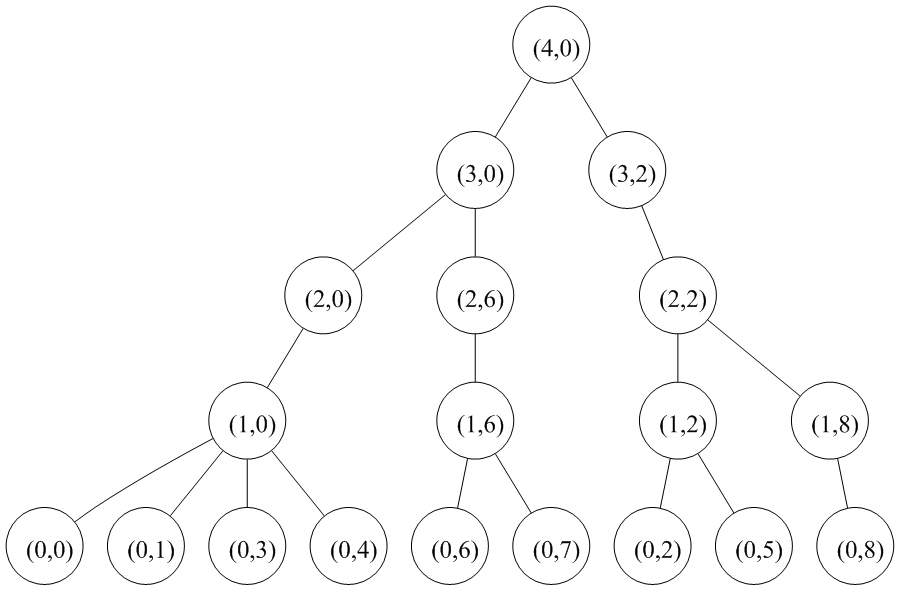
\includegraphics[width=10cm]{ipfs/ipfs-forest-layercloning-a-hierarchy.png}}%
	%
	\\
	%
	\subfigure[After cloning layer 2]
	{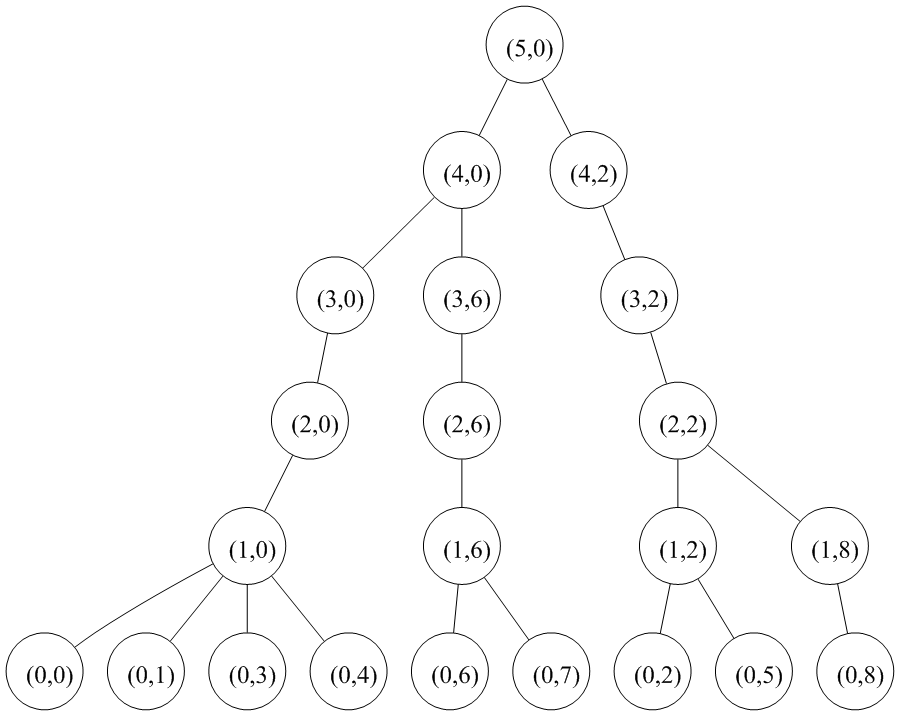
\includegraphics[width=10cm]{ipfs/ipfs-forest-layercloning-b-hierarchy.png}}%
\caption{An example of layer cloning.}
\label{fig:ipfs-forest-layercloning}
\end{stusubfig}
%---

\paragraph{C++ Method Interface}

\begin{lstlisting}[style=Prototype]
void clone_layer(int indexB);
\end{lstlisting}

\paragraph{User Interface for Image Analysis}

The simplest user interface just allows the user to clone the current layer by (for example) clicking on a menu item (see Figure~\ref{fig:ipfs-forest-layercloning-gui}). After cloning the layer, the interface can display the clone so that the user can begin working with it immediately. An alternative would be to allow the user to clone any layer in the forest by displaying a dialog box allowing them to choose the layer to be cloned, but in my view the former approach is more intuitive.

%---
\stufigex{height=6cm}{ipfs/ipfs-forest-layercloning-gui.png}{The user interface for layer cloning: a simple menu item allowing the current layer to be cloned.}{fig:ipfs-forest-layercloning-gui}{p}
%---

\paragraph{Precondition Checking}

The only precondition that needs checking for layer cloning is that the clonee (the layer being cloned) exists. This can be trivially checked in $O(1)$ time. Note that if the clone layer command is invoked from the user interface, the layer will inevitably exist (and we can skip the check), since the layer currently being viewed exists by definition.

\paragraph{Executing the Command}

Pseudo-code to execute a clone layer command is shown in Listing~\ref{code:ipfs-forest-clonelayerimpl}. The essence of the approach taken is simple: clone the graph of the layer below, then update the forest links between the clone layer and the layers below and above it. In order to implement the algorithm efficiently, however, it is important to employ a sensible iterator-based interface to the nodes in each forest layer: this allows us to iterate over the nodes in a layer in linear time and avoid the costly node lookups that might otherwise be necessary. Thus, in the pseudo-code, we iterate simultaneously over the nodes in the clonee layer and the clone, first propagating each parent link from the clonee node up to the clone node, then linking the corresponding nodes in the clonee and the clone together.

To analyse the complexity of the algorithm (referring to the listing), we proceed as follows. Firstly, let $L$ be the number of existing layers prior to the clone operation, and let $n_\ell$ be the number of nodes and $e_\ell$ be the number of adjacency graph edges in layer $\ell$. Let the clone layer being inserted be layer $c$ and the layer below it (from which it was cloned) be layer $b$. Then evidently $n_c = n_b$ and $e_c = e_b$.

Line $8$ is $O(1)$, because it only involves an array lookup. The complexity of Line $9$ differs depending on whether $b$ is a branch layer or the leaf layer. If it is a branch layer, then cloning the nodes in the graph is $O(n_b)$ and cloning the edges is $O(e_b)$, since these just involve cloning a tree-based data structure such as a std::map, which can be done in linear time. If $b$ is the leaf layer, then cloning the nodes is slightly trickier, because we need to create a std::map (the branch layer's representation for nodes) from a std::vector (the leaf layer's representation). However, as no sorting is actually required, this can still in principle be done in $O(n_b)$ time using a divide and conquer approach (na\"ive implementations, however, are more likely to end up being $O(\log (n_b!))$\footnote{Since $\log 1 + \ldots + \log n_b = \log (1 \times \ldots \times n_b) = \log (n_b!)$. It is worth noting in passing that -- despite the impression potentially given by the factorial -- this is actually somewhat better than $O(n_b \log n_b)$.}). Cloning the edges is harder, because sorting may be required, although for regular grids it is in principle possible to devise a suitable scheme to traverse the edges in sorted order. If sorting can be avoided in this way, then cloning the edges takes $O(e_b)$; if not, it takes $O(\log (e_b!))$. The total cost of Line $9$ is thus $O(n_b + e_b)$ when cloning a branch layer, and at worst $O(\log (n_b!) + \log (e_b!))$ when cloning the leaf layer. Provided that $b$'s adjacency graph is connected (as are all the adjacency graphs dealt with in this thesis), $n_b \in O(e_b)$, in which case this simplifies to $O(e_b)$ for the branch layer case, and $O(\log (e_b!))$ for the leaf layer case. Line $10$ is amortised $O(1)$, but for an individual operation can be $O(L)$ -- however, $L$ is generally a very small number. Lines $14-17$ are $O(1)$. Lines $19-23$ are $O(n_c) = O(n_b)$, since each iteration of the loop does a constant amount of work. In total, then the algorithm as a whole is (amortised) $O(e_b)$ in the branch layer case, and (amortised) $O(\log (e_b!))$ in the leaf layer case.

%---
\begin{stulisting}[p]
\caption{Forest : Layer Cloning : Execution}
\label{code:ipfs-forest-clonelayerimpl}
\lstinputlisting[style=Default]{ipfs/ipfs-forest-clonelayerimpl.lst}
\end{stulisting}
%---

\paragraph{Undoing the Command}

A clone layer command can be undone by simply deleting the clone (see Listing~\ref{code:ipfs-forest-deletelayerimpl} for pseudo-code). The complexity of this is analysed in the next section.

\afterpage{\clearpage}
\newpage

%~~~~~~~~~~~~~~~~~~~~~~~~~~~~~~~~~~~~~~~~~~~~~~~~
\subsubsection{Layer Deletion}
%~~~~~~~~~~~~~~~~~~~~~~~~~~~~~~~~~~~~~~~~~~~~~~~~

\paragraph{Description}

Any layer except the lowest can be deleted from the hierarchy (for example, see Figure~\ref{fig:ipfs-forest-layerdeletion}). In terms of the partition forest definition, this has the effect of removing both the specified partitioning graph from $\textit{PG}$ and the forest links referencing the deleted layer from $\textit{FL}$, and adding new forest links where necessary between any layers on either side of the one being removed.

%---
\begin{stusubfig}{p}
	\subfigure[Before deleting layer 1]
	{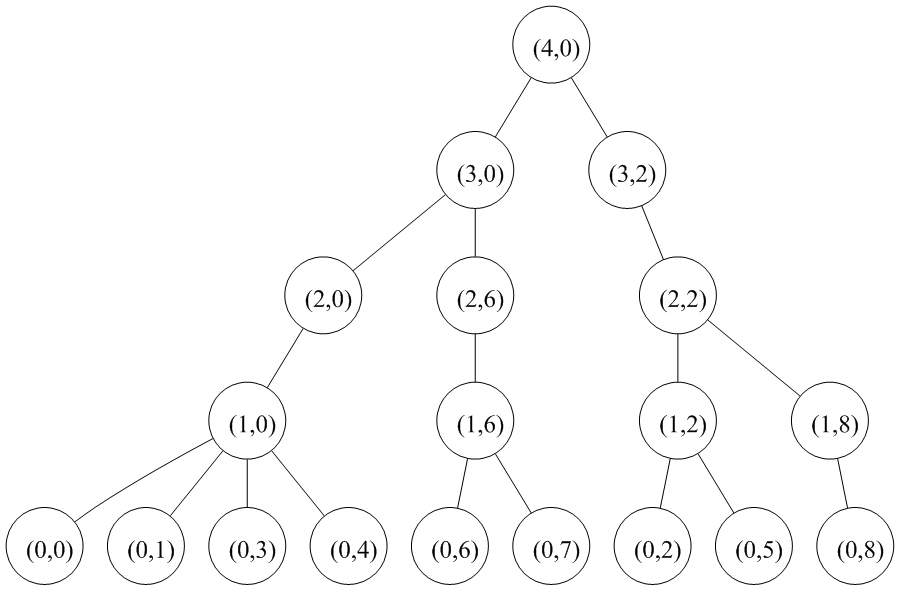
\includegraphics[width=10cm]{ipfs/ipfs-forest-layerdeletion-a-hierarchy.png}}%
	%
	\\
	%
	\subfigure[After deleting layer 1]
	{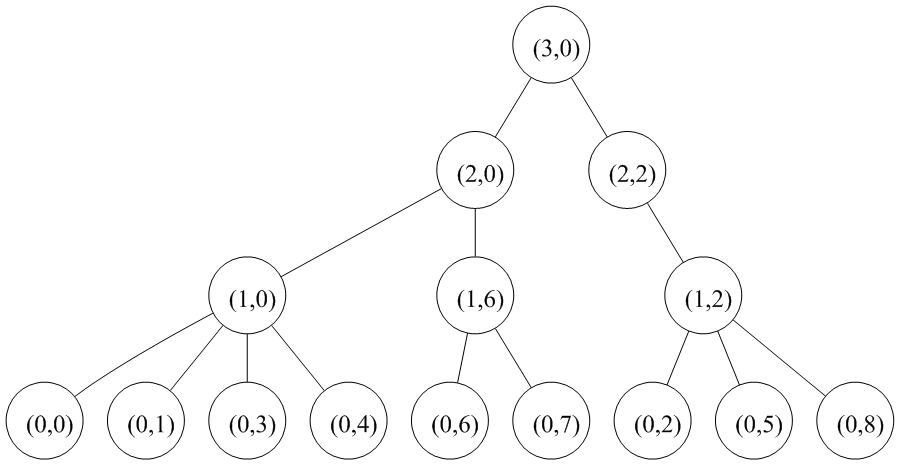
\includegraphics[width=10cm]{ipfs/ipfs-forest-layerdeletion-b-hierarchy.png}}%
\caption{An example of layer deletion.}
\label{fig:ipfs-forest-layerdeletion}
\end{stusubfig}
%---

\paragraph{C++ Method Interface}

\begin{lstlisting}[style=Prototype]
void delete_layer(int indexD);
\end{lstlisting}

\paragraph{User Interface for Image Analysis}

As with layer cloning, the simplest user interface just allows the user to delete the current layer by clicking on a menu item (see Figure~\ref{fig:ipfs-forest-layerdeletion-gui}).

%---
\stufigex{height=5cm}{ipfs/ipfs-forest-layerdeletion-gui.png}{The user interface for layer deletion: a simple menu item allowing the current layer to be deleted.}{fig:ipfs-forest-layerdeletion-gui}{p}
%---

\paragraph{Precondition Checking}

The only precondition that needs checking for layer deletion is that the layer being deleted is a branch layer. This is trivial to check in $O(1)$ time. (Depending on the design of the overall application, it may be necessary to make layer deletion slightly more constrained. For instance, an application that shows only branch layers may want to prevent the user from deleting the last branch layer, even though it's perfectly fine when viewed strictly from a partition forest perspective. Regardless, though, the required checks remain trivial.)

\paragraph{Executing the Command}

Pseudo-code to execute a delete layer command is shown in Listing~\ref{code:ipfs-forest-deletelayerimpl}. The idea is to update the forest links between the layers on either side of the layer to be deleted and then remove the layer itself from the forest. Specifically, if $D$ is the layer being deleted, $B$ is the layer below it and $A$ is the layer above (if it exists), then each node in $B$ should have its parent link updated to point to its grandparent in layer $A$. The grandparent nodes in $A$ should similarly have their child links updated to point to their grandchildren in layer $B$. To implement this efficiently, it is important to avoid calculating the grandchildren of nodes in $A$ explicitly. This is most easily arranged by iterating over the grandchildren and updating the grandparents during the course of the iteration (see pseudo-code). It is important to return the deleted layer (unchanged) at the end of the process, because it must be cached if we are to support undo.

We use the same notation to analyse the complexity as in the layer cloning analysis. Referring to the listing, line $16$ is a simple $O(1)$ array lookup. Lines $17-19$ are $O(n_a)$, since each iteration (if the loop happens at all) does a constant amount of work for each node in layer $A$. Lines $21-22$ are simple $O(1)$ array lookups. Lines $23-27$ are $O(n_b (\log n_d + \log n_a + \log \#\mathit{children}(\mathit{grandparentA}))) = O(n_b \log n_d)$, since $n_a \le n_d$ and $\#\mathit{children}(\mathit{grandparentA}) \le n_d$. Line $29$ is amortised $O(1)$. The algorithm as a whole is $O(n_a + n_b \log n_d) = O(n_b \log n_d)$, since $n_a \le n_b$.

%---
\begin{stulisting}[p]
\caption{Forest : Layer Deletion : Execution}
\label{code:ipfs-forest-deletelayerimpl}
\lstinputlisting[style=Default]{ipfs/ipfs-forest-deletelayerimpl.lst}
\end{stulisting}
%---

\paragraph{Undoing the Command}

%---
\begin{stulisting}[p]
\caption{Forest : Layer Deletion : Undo}
\label{code:ipfs-forest-undeletelayerimpl}
\lstinputlisting[style=Default]{ipfs/ipfs-forest-undeletelayerimpl.lst}
\end{stulisting}
%---

Pseudo-code to undo a delete layer command is shown in Listing~\ref{code:ipfs-forest-undeletelayerimpl}. The algorithm reinserts the deleted layer $D$ (cached during deletion) back into the forest, then recreates the forest links in the layers below ($B$) and above ($A$, where applicable) the deletion point, using the links in the deleted layer to discover which links to add.

(It is worth observing that undeleting a layer in an interactive system may not necessarily be as simple as this. One good reason for deleting a layer is to save memory, in particular the substantial amount of memory associated with the textures that display the partition forest to the user. Caching these textures when deleting a layer would in this case defeat the point of deleting the layer in the first place. A compromise solution is to cache the layer itself, but delete the textures -- we then arrange to recreate the textures from scratch in the event that the layer is undeleted.)

In terms of complexity, line $8$ in the listing is amortised $O(1)$. Lines $12-15$ are $O(n_a)$, because they involve a simple array lookup, followed by at most a constant time operation for each node in layer $A$. Line $17$ is a simple $O(1)$ array lookup. Lines $18-21$ are more interesting: note that line $20$, which involves an $O(\log n_b)$ lookup, executes exactly $n_b$ times (we're running through the children of every node in the layer above $B$, i.e.~through all the nodes actually in $B$), so the cost of the first part of the loop is $O(n_b \log n_b)$. Line $21$, by contrast, executes $n_d$ times and involves at most $O(\log n_a + \log \#\mathit{children}(\mathit{n.parent()}))$ amount of work each time, adding $O(n_d (\log n_a + \log \#\mathit{children}(\mathit{n.parent()})))$ work to the total. This is dominated by the earlier $O(n_b \log n_b)$, which is thus the total cost of lines $18-21$. The cost of the entire algorithm, bearing in mind that line $8$'s cost was amortised, and that $n_a \le n_b$, is thus amortised $O(n_b \log n_b)$.

\afterpage{\clearpage}
\newpage

%~~~~~~~~~~~~~~~~~~~~~~~~~~~~~~~~~~~~~~~~~~~~~~~~
\subsubsection{Sibling Node Merging}
%~~~~~~~~~~~~~~~~~~~~~~~~~~~~~~~~~~~~~~~~~~~~~~~~

\paragraph{Description}

Sibling nodes in any layer of the hierarchy other than the lowest can be merged provided that the union of the objects they represent is contiguous (this condition ensures that the new node post-merging still represents a valid object). A set of nodes are siblings if they either all have the same parent, or all have no parent (the latter case occurs when the nodes are in the top layer of the hierarchy, when they are all implicitly children of the top-level object represented by the partition forest -- e.g.~the whole image in the case of an image partition forest). The algorithm takes as input the set of sibling nodes to be merged, and returns the node resulting from the merge. An example is shown in Figure~\ref{fig:ipfs-forest-siblingnodemerging}.

%---
\begin{stusubfig}{p}
	\subfigure[The forest before the merge.]
	{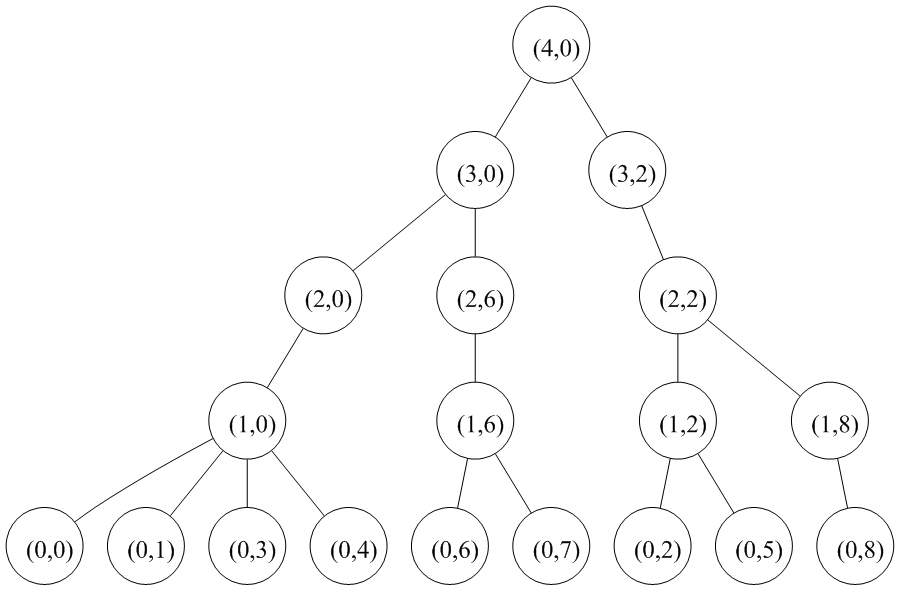
\includegraphics[width=.45\linewidth]{ipfs/ipfs-forest-siblingnodemerging-a-hierarchy.png}}%
	%
	\hspace{8mm}%
	%
	\subfigure[The layer 2 graph before the merge.]
	{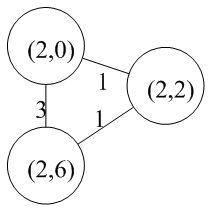
\includegraphics[width=.2\linewidth]{ipfs/ipfs-forest-siblingnodemerging-a-graph2.png}}%
	%
	\hspace{8mm}%
	%
	\subfigure[The forest after the merge.]
	{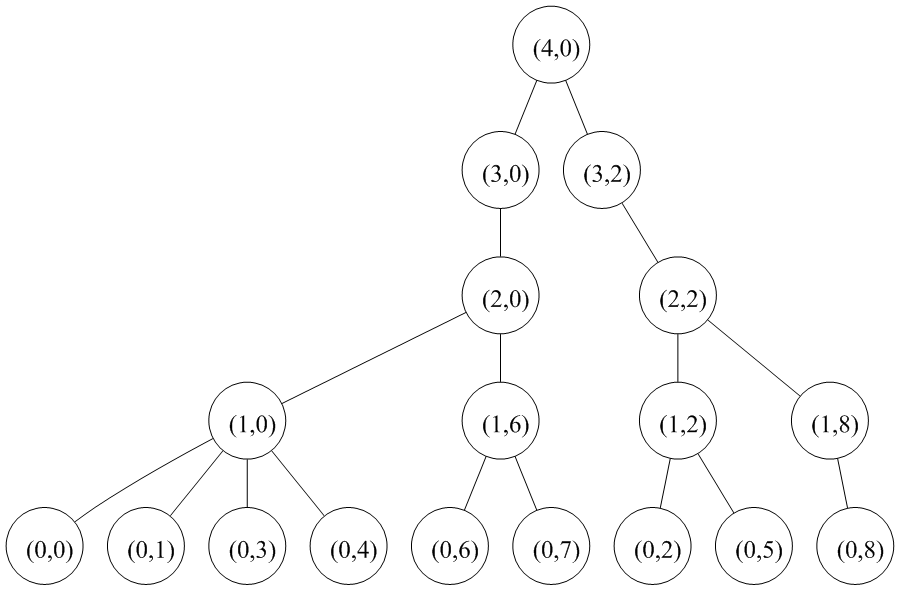
\includegraphics[width=.45\linewidth]{ipfs/ipfs-forest-siblingnodemerging-b-hierarchy.png}}%
	%
	\hspace{8mm}%
	%
	\subfigure[The layer 2 graph after the merge.]
	{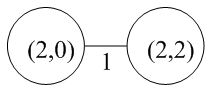
\includegraphics[width=.2\linewidth]{ipfs/ipfs-forest-siblingnodemerging-b-graph2.png}}%
\caption{An example of sibling node merging: merging nodes (2,0) and (2,6).}
\label{fig:ipfs-forest-siblingnodemerging}
\end{stusubfig}
%---

\paragraph{C++ Method Interface}

\begin{lstlisting}[style=Prototype]
NodeID merge_sibling_nodes(const set<NodeID>& nodes);
\end{lstlisting}

\paragraph{User Interface for Image Analysis}

Although it is a crucial operation, it doesn't make sense to expose sibling-only node merging in the interface, since that would require the user to keep track of which nodes share the same forest parent. A much better solution (shown later) is to expose the more intuitive operation that merges arbitrary nodes in the same layer into their connected components.

\paragraph{Precondition Checking}

The following preconditions must be checked for sibling node merging (see the pseudo-code in Listing~\ref{code:ipfs-forest-mergesiblingnodes} for the method):

\begin{enumerate}

\item There must be more than one node to be merged. (This can be trivially checked in $O(1)$ time.)
\item None of the nodes must be in the lowest layer of the forest. (This can be checked in time $O(k)$, where $k$ is the number of nodes.)
\item The nodes must share a common parent in the forest. Note that this implies that they must all be in the same layer. (Assuming the $k$ nodes share a common layer $\ell$, then the cost of looking up the parent for each node is $O(\log n_\ell)$, whence the total cost of this check is $O(k \log n_\ell)$.)
\item The union of the objects represented by the nodes to be merged must be connected. (This can be checked in $O(k \log e_\ell)$ time. To see this, examine the \texttt{are_connected} and \texttt{find_connected_component} listings in Appendix~\ref{chap:appendixpf}. The worst case is when all the nodes must be visited, i.e.~when there is a single connected component. When that happens, over the course of the process, every node is erased from the set of input nodes and inserted into the set of result nodes -- $O(\log (k!))$ overall. Each node is also pushed onto the queue and popped off it again -- $O(k)$ overall. Every node but the seed is also looked up during the \texttt{contains} call -- $O(\log (k!))$ overall, because the size of the input node set decreases after each such call. The dominant cost of $O(k \log e_\ell)$ comes from having to look up the adjacent edges for each input node in the tree-based data structure storing the edges for forest layer $\ell$.)

\end{enumerate}

\noindent The overall cost of checking the preconditions is thus $O(k \log e_\ell)$, since $n_\ell \in O(e_\ell)$ (the adjacency graphs we're dealing with are connected).

%---
\begin{stulisting}[p]
\caption{Forest : Sibling Node Merging : Precondition Checking}
\label{code:ipfs-forest-mergesiblingnodes}
\lstinputlisting[style=Default]{ipfs/ipfs-forest-mergesiblingnodes.lst}
\end{stulisting}
%---

%---
\begin{stulisting}[p]
\caption{Forest : Sibling Node Merging : Command}
\label{code:ipfs-forest-mergesiblingnodescommand}
\lstinputlisting[style=Default]{ipfs/ipfs-forest-mergesiblingnodescommand.lst}
\end{stulisting}
%---

\paragraph{Executing the Command}

Pseudo-code to execute a sibling node merge command is shown in Listing~\ref{code:ipfs-forest-mergesiblingnodesimpl}. Firstly, the mergee node with the lowest index is picked to be the result of the merge (for instance, nodes $(2,2)$, $(2,1)$ and $(2,5)$ in a hypothetical forest would be merged into a new node called $(2,1)$, since $\min(\{2,1,5\}) = 1$). This node is referred to as the `canonical' node in the code.

In Step 1, forest links are then added (in both directions) between the canonical node and the children of the other nodes being merged (the parent links from the children to the canonical node replace those already there; the child links in the other direction are simply added). If the nodes being merged are not in the highest layer, the forest links joining the non-canonical nodes to their common parent must also be removed (since the non-canonical nodes will ultimately be removed from the forest).

As a result of merging the other nodes into the canonical node, the latter may gain new edges that it did not have before (since some of the other nodes may have been adjacent to nodes that it itself was not), and its properties (such as its voxel count) will generally change. In Step 2, therefore, its edges are updated using the edges of the other nodes. When there is a duplicate edge (i.e.~both the canonical node and one of the other nodes have an edge to a third node), then a new edge weight has to be chosen -- depending on the scheme in use, this might for example involve taking the minimum of the weights on the two existing edges (the appropriate method for a lowest pass point approach). Also in Step 2, the canonical node's properties are recalculated directly from those of its children (note that this is why the partition forest definition places direct calculability constraints on property sets).

Finally, Step 3 removes the non-canonical nodes. In the pseudo-code given (based on my implementation in \emph{millipede}), this also has the effect of removing any edges adjacent to those nodes -- if an alternative implementation strategy is chosen, however, these may need to be removed manually.

TODO: Complexity analysis

%---
\begin{stulisting}[p]
\caption{Forest : Sibling Node Merging : Execution}
\label{code:ipfs-forest-mergesiblingnodesimpl}
\lstinputlisting[style=Default]{ipfs/ipfs-forest-mergesiblingnodesimpl.lst}
\end{stulisting}
%---

\paragraph{Undoing the Command}

To undo a sibling node merge command, the intuition is that the node resulting from the merge must be split back into the nodes that were originally merged to create it. As we will see in the next section, however, a node is split not by specifying the \emph{nodes} into which to split it (these do not exist prior to the split, so that approach doesn't work), but by specifying connected groups of the node's children: a parent is generated for each of these groups and the node to be split is replaced with the group parents. For that reason, if we want to be able to undo a sibling node merge then we must store the children of each of the nodes to be merged when we initially execute the command. The merge can then be undone by splitting the merge result back into the components specified by the stored child groups (see Listing~\ref{code:ipfs-forest-mergesiblingnodescommand} for the detailed implementation).

\afterpage{\clearpage}
\newpage

%~~~~~~~~~~~~~~~~~~~~~~~~~~~~~~~~~~~~~~~~~~~~~~~~
\subsubsection{Node Splitting}
%~~~~~~~~~~~~~~~~~~~~~~~~~~~~~~~~~~~~~~~~~~~~~~~~

\paragraph{Description}

Nodes in any layer of the hierarchy other than the lowest can be split into multiple nodes representing smaller objects. (Note that the definition of objects requires that each of these smaller objects must be contiguous.) The algorithm takes as input the node to be split, and a set of groups of the node's children into which to split it, where each group is a set of child nodes. It returns the nodes created by the split. An example is shown in Figure~\ref{fig:ipfs-forest-nodesplitting}.

%---
\begin{stusubfig}{p}
	\subfigure[The forest before the split.]
	{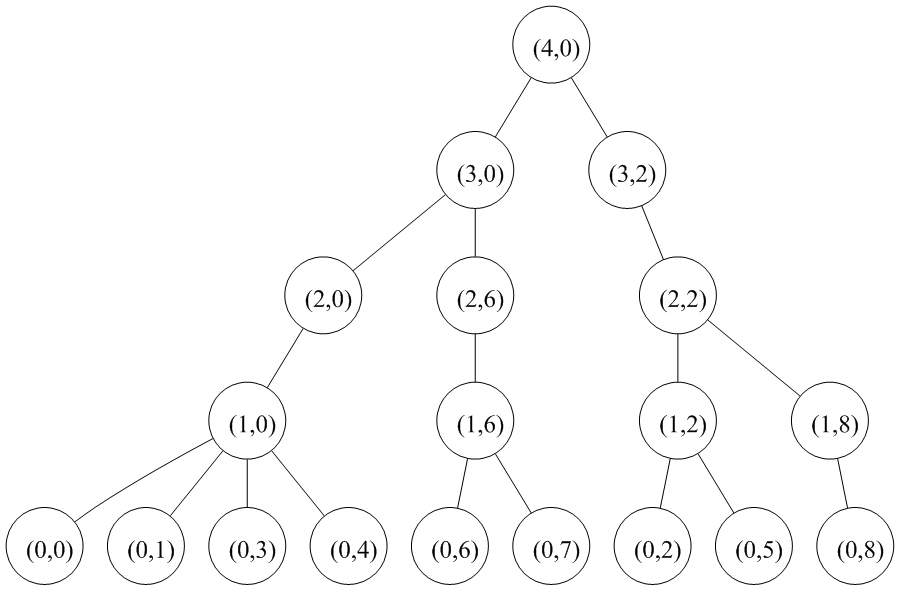
\includegraphics[width=.45\linewidth]{ipfs/ipfs-forest-nodesplitting-a-hierarchy.png}}%
	%
	\hspace{8mm}%
	%
	\subfigure[The layer 1 graph before the split.]
	{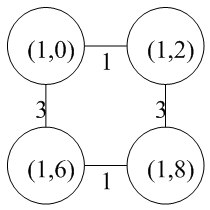
\includegraphics[width=.2\linewidth]{ipfs/ipfs-forest-nodesplitting-a-graph1.png}}%
	%
	\hspace{8mm}%
	%
	\subfigure[The forest after the split.]
	{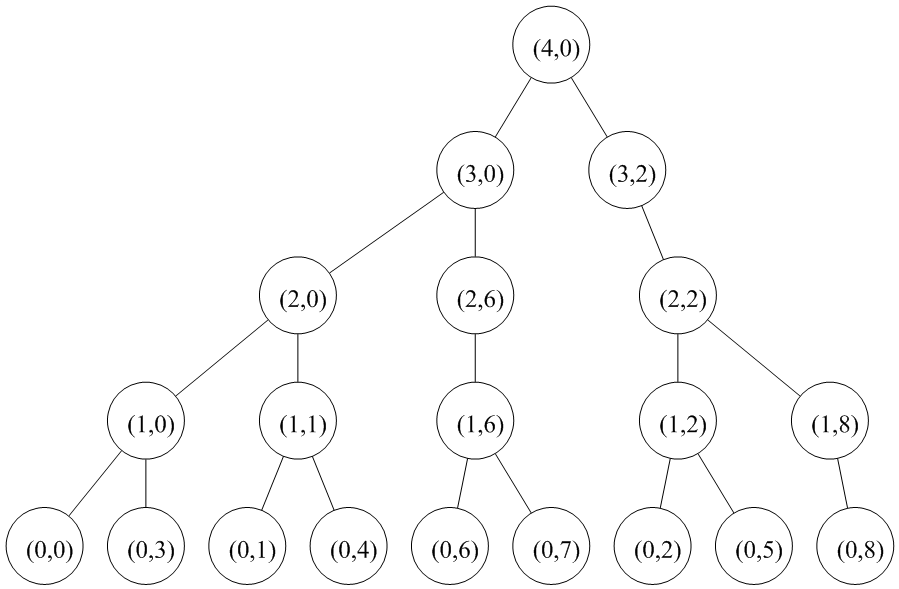
\includegraphics[width=.45\linewidth]{ipfs/ipfs-forest-nodesplitting-b-hierarchy.png}}%
	%
	\hspace{8mm}%
	%
	\subfigure[The layer 1 graph after the split.]
	{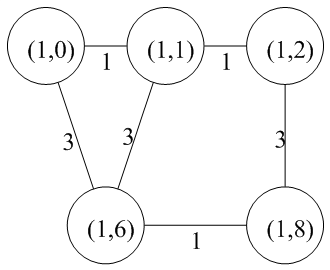
\includegraphics[width=.2\linewidth]{ipfs/ipfs-forest-nodesplitting-b-graph1.png}}%
\caption{An example of node splitting: splitting node (1,0) into two.}
\label{fig:ipfs-forest-nodesplitting}
\end{stusubfig}
%---

\paragraph{C++ Method Interface}

\begin{lstlisting}[style=Prototype]
set<NodeID> split_node(const NodeID& node,
                       const vector<set<int> >& groups);
\end{lstlisting}

\paragraph{User Interface for Image Analysis}

The user interface for node splitting is necessarily more complicated than that for earlier operations, because the user needs to be able to indicate the way in which a node should be split. As illustrated in Figure~\ref{fig:ipfs-forest-nodesplitting-gui}, this is a multi-step operation. The user initially selects and marks a node to be split, then defines the components into which it should be split by iteratively selecting and marking connected subgroups of its children. (If a mistake is made, it is possible to remove a subgroup and try again, although this is not illustrated for space reasons.) As the illustrated example implies, any remaining unmarked children will be automatically divided into subgroups by finding their connected components (this substantially reduces the work that has to be done by the user). Finally, the user `finalizes' the split and the desired changes are made to the forest.

%---
\begin{stusubfig}{p}
	\subfigure[Select the node to be split in the forest]
	{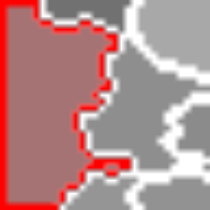
\includegraphics[width=.2\linewidth]{ipfs/ipfs-forest-nodesplitting-gui-a.png}}%
	%
	\hspace{8mm}%
	%
	\subfigure[Mark it to be split by clicking the menu item]
	{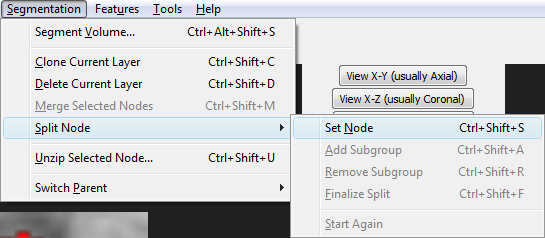
\includegraphics[width=.5\linewidth]{ipfs/ipfs-forest-nodesplitting-gui-b.png}}%
	%
	\hspace{8mm}%
	%
	\subfigure[After marking it, its children will be highlighted]
	{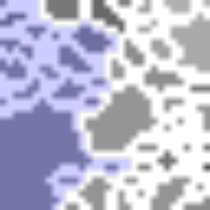
\includegraphics[width=.2\linewidth]{ipfs/ipfs-forest-nodesplitting-gui-c.png}}%
	%
	\hspace{8mm}%
	%
	\subfigure[Select the child nodes in a subgroup]
	{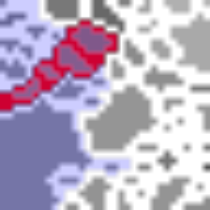
\includegraphics[width=.2\linewidth]{ipfs/ipfs-forest-nodesplitting-gui-d.png}}%
	%
	\hspace{8mm}%
	%
	\subfigure[Add the subgroup by clicking the menu item]
	{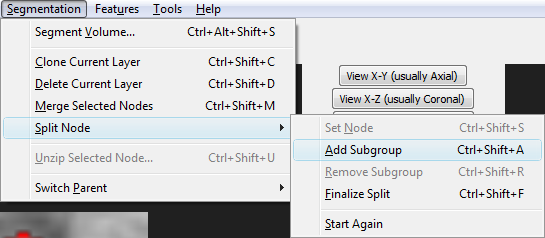
\includegraphics[width=.5\linewidth]{ipfs/ipfs-forest-nodesplitting-gui-e.png}}%
	%
	\hspace{8mm}%
	%
	\subfigure[Each subgroup will be assigned a different colour]
	{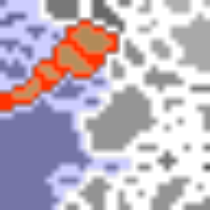
\includegraphics[width=.2\linewidth]{ipfs/ipfs-forest-nodesplitting-gui-f.png}}%
	%
	\hspace{8mm}%
	%
	\subfigure[Repeat (d)-(f) to add other subgroups, then finalize the split by clicking the menu item]
	{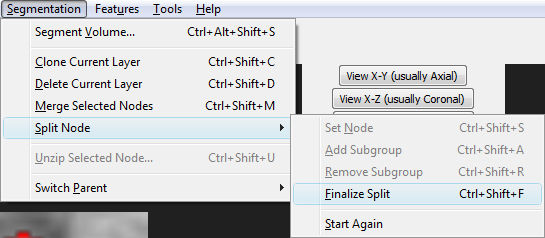
\includegraphics[width=.5\linewidth]{ipfs/ipfs-forest-nodesplitting-gui-g.png}}%
	%
	\hspace{8mm}%
	%
	\subfigure[The node will be split as indicated]
	{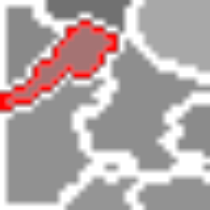
\includegraphics[width=.2\linewidth]{ipfs/ipfs-forest-nodesplitting-gui-h.png}}%
\caption{The user interface for node splitting}
\label{fig:ipfs-forest-nodesplitting-gui}
\end{stusubfig}
%---

\paragraph{Precondition Checking}

The following preconditions must be checked for node splitting (see the pseudo-code in Listing~\ref{code:ipfs-forest-splitnode} for the method):

\begin{enumerate}

\item The node to be split must not be in the leaf layer of the forest. (This can be trivially checked in $O(1)$ time.)
\item The node to be split must exist. (This can be checked in $O(1)$ time for the leaf layer, and $O(\log n_\ell)$ time for branch layer $\ell$.)
\item There must be more than one subgroup. (This can be trivially checked in $O(1)$ time.)
\item The subgroups must partition the children of the node being split. (This can be checked in time $O(\log C!)$, where $C$ is the number of children, since each inner loop iteration involves a logarithmic amount of work on a set whose size decreases linearly from $C$ to $1$, and $\sum_{i=1}^C \log i = \log C!$.)
\item Each of the subgroups must be non-empty and connected. (Each of the $G$ groups requires $O(1)$ time for the non-empty check, and TODO.)

\end{enumerate}

When implementing node splitting in a user interface like the one described above, these preconditions should be checked by the interface, not by the forest at the time of finalizing the split. The user should not, for example, have the option of adding invalid subgroups or finalizing a split without defining any subgroups.

%---
\begin{stulisting}[p]
\caption{Forest : Node Splitting : Precondition Checking}
\label{code:ipfs-forest-splitnode}
\lstinputlisting[style=Default]{ipfs/ipfs-forest-splitnode.lst}
\end{stulisting}
%---

\paragraph{Executing the Command}

Pseudo-code to execute a split node command is shown in Listing~\ref{code:ipfs-forest-splitnodeimpl}. In Step 1, the node to be split is deleted from the forest -- this involves removing the forest links that connect the node to its parent and children, and removing the node itself from the partitioning graph for its forest layer (in the pseudo-code, removing the node from the graph also removes its adjacent edges). In Step 2, each of the groups of children that define a node resulting from the split is used to generate a new node in the split layer (a parent for the group). This new node has the index of the lowest-indexed child node (for instance, the parent of nodes $(1,5)$, $(1,3)$ and $(1,7)$ in a hypothetical forest would be denoted $(2,3)$). Its properties are calculated by combining those of its children in the usual way. Forest links are added to connect the new node to its children in the group and its parent in the layer above (namely the parent of the node that is being split). Finally, in Step 3, the adjacency graph for the split layer is locally reconstructed around the nodes resulting from the split (it was locally destroyed when the node being split was removed) -- this is done by considering all the edges adjacent to any of the split node's children, and propagating them upwards to the split layer. For instance, if node $p_1$ in the split layer has children $c_1$ and $c_2$, and node $p_2$ in the split layer has children $c_3$ and $c_4$, and the only edges between children of $p_1$ and $p_2$ are $(\{c_1,c_3\}, w_{13})$ and $(\{c_2,c_4\}, w_{24})$, then this induces an edge $(\{p_1,p_2\}, f(w_{13}, w_{24}))$ in the split layer, where $f$ is some appropriate function on edge weights, such as $\min$ in the case of a lowest pass point approach.

TODO: Complexity analysis

%---
\begin{stulisting}[p]
\caption{Forest : Node Splitting : Execution}
\label{code:ipfs-forest-splitnodeimpl}
\lstinputlisting[style=Default]{ipfs/ipfs-forest-splitnodeimpl.lst}
\end{stulisting}
%---

\paragraph{Undoing the Command}

To undo a split node command, it is enough to just re-merge the results of the split using a sibling node merge (see Listing~\ref{code:ipfs-forest-mergesiblingnodesimpl} for pseudo-code).

\afterpage{\clearpage}
\newpage

%################################################
\subsection{Zipping Algorithms}
%################################################

Whilst the core mutating algorithms provide all that is theoretically required for partition forest editing, certain operations are nevertheless tedious for the user to perform using only these primitives. For instance, it seems intuitively sensible that the user should be able to merge not only nodes that are siblings in the forest, but any nodes that are adjacent in the graph for their forest layer. Such `higher-level' algorithms, however, require more substantial changes to the structure of the forest; in particular, they require changes to be made in more than one layer.

In order to facilitate the implementation of such algorithms, it is helpful to introduce two intermediary forest operations that I call \emph{unzip node} (or just \emph{unzipping}) and \emph{zip chains} (or just \emph{zipping}). These are respectively multi-layer split and merge operations on the forest, and can be implemented in terms of their lower-level counterparts. In fact, such an approach is not only possible but advisable, since it can be used to avoid writing special code to undo the operations. The key is to introduce an entity called a \emph{listener-alerting command sequence guard}. This is created at the start of a composite operation like an unzip, and informs both the application's command manager and any listeners that a command sequence is about to start (in C++, this would happen in the constructor for the guard). The relevant lower-level commands are then executed, after which the guard is destroyed again, informing the application's command manager and any listeners that the command sequence has ended (in C++, this would happen in the guard's destructor). Undoing the composite operation is then a simple matter of undoing the lower-level commands in reverse order, something that can be easily handled by any decent command manager implementation. Bearing this in mind, we can now examine each of the zipping algorithms in detail.

\newpage

%~~~~~~~~~~~~~~~~~~~~~~~~~~~~~~~~~~~~~~~~~~~~~~~~
\subsubsection{Unzipping}
%~~~~~~~~~~~~~~~~~~~~~~~~~~~~~~~~~~~~~~~~~~~~~~~~

\paragraph{Description}

A node in any layer of the hierarchy can be unzipped to a specified higher layer (or the top of the hierarchy). This essentially `separates out' the branch from the higher layer down to the specified node: it is effectively a multi-layer split, with a set containing the node in question as one of the groups at each stage. The key issue that has to be addressed in order to make this work is the need to find the other groups for each split: the algorithm presented here solves this problem by defining the other groups to be the connected components of what is left after removing the node being unzipped from consideration. See Figure~\ref{fig:ipfs-forest-unzipping} for an example.

%---
\begin{stusubfig}{p}
	\subfigure[Initial hierarchy]{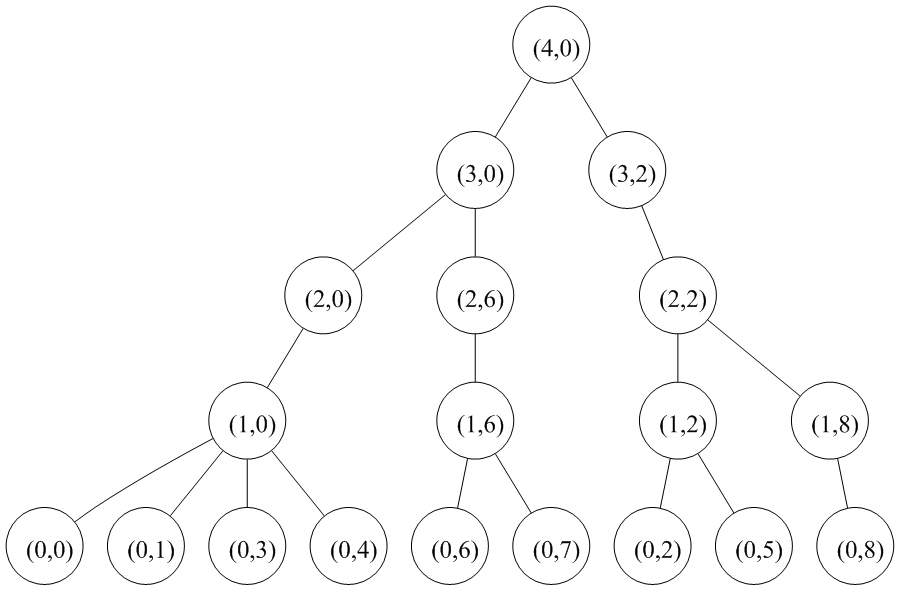
\includegraphics[width=.45\linewidth]{ipfs/ipfs-forest-unzipping-a-hierarchy.png}}%
	\hspace{8mm}%
	\subfigure[After splitting $(1,2)$]{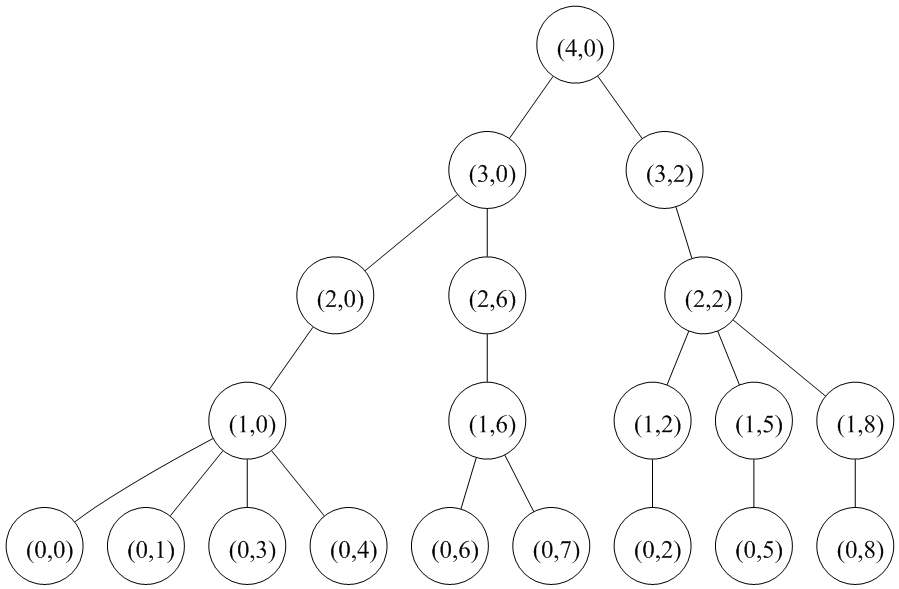
\includegraphics[width=.45\linewidth]{ipfs/ipfs-forest-unzipping-b-hierarchy.png}}%
	\\
	\subfigure[After splitting $(2,2)$]{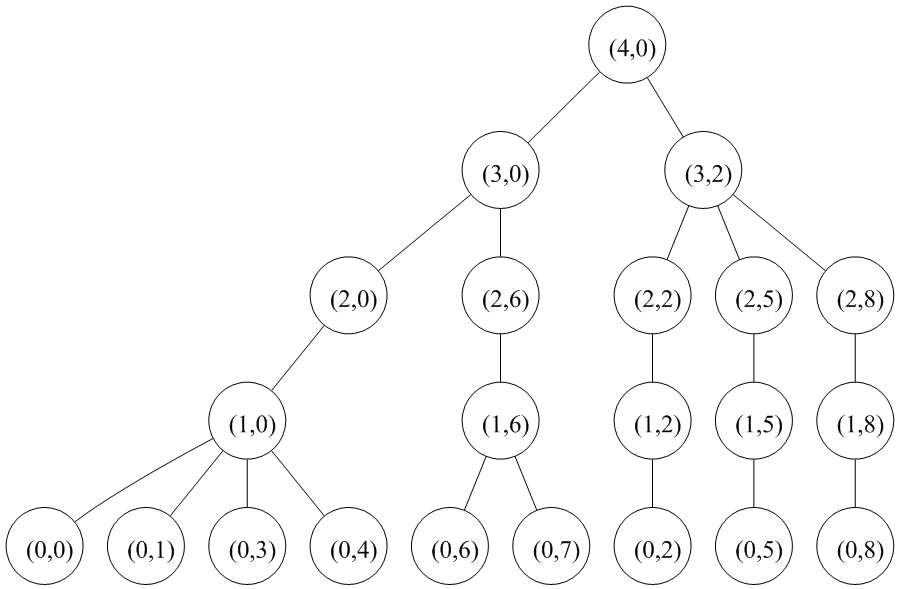
\includegraphics[width=.45\linewidth]{ipfs/ipfs-forest-unzipping-c-hierarchy.png}}%
	\hspace{8mm}%
	\subfigure[After splitting $(3,2)$]{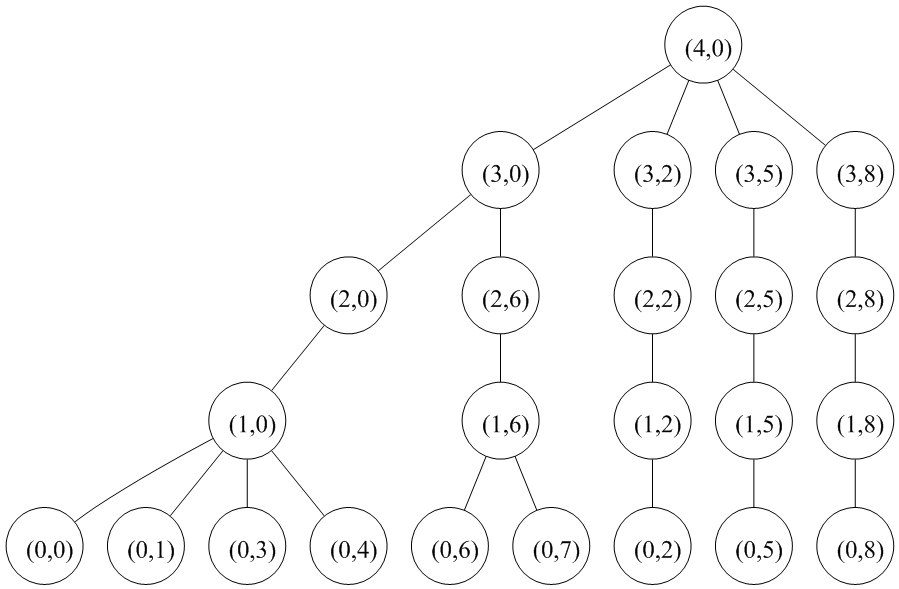
\includegraphics[width=.45\linewidth]{ipfs/ipfs-forest-unzipping-d-hierarchy.png}}%
	\\
	\subfigure[Initial layer $1$ graph]{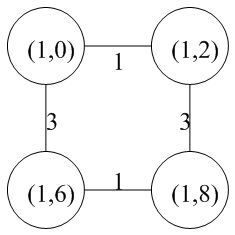
\includegraphics[width=.22\linewidth]{ipfs/ipfs-forest-unzipping-a-graph1.png}}%
	\hspace{8mm}%
	\subfigure[Initial layer $2$ graph]{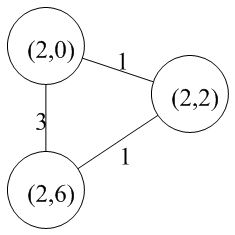
\includegraphics[width=.22\linewidth]{ipfs/ipfs-forest-unzipping-a-graph2.png}}%
	\hspace{8mm}%
	\subfigure[Initial layer $3$ graph]{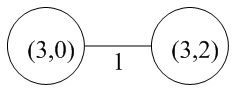
\includegraphics[width=.22\linewidth]{ipfs/ipfs-forest-unzipping-a-graph3.png}}%
	\\
	\subfigure[Resulting layer $1$ graph]{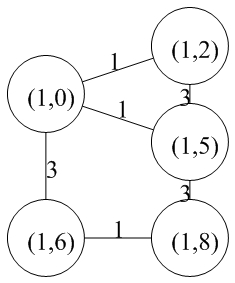
\includegraphics[width=.22\linewidth]{ipfs/ipfs-forest-unzipping-b-graph1.png}}%
	\hspace{8mm}%
	\subfigure[Resulting layer $2$ graph]{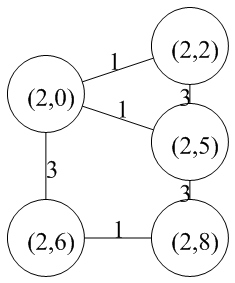
\includegraphics[width=.22\linewidth]{ipfs/ipfs-forest-unzipping-c-graph2.png}}%
	\hspace{8mm}%
	\subfigure[Resulting layer $3$ graph]{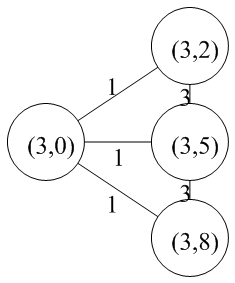
\includegraphics[width=.22\linewidth]{ipfs/ipfs-forest-unzipping-d-graph3.png}}%
\caption{An example of unzipping: unzipping node $(0,5)$ to layer $3$}
\label{fig:ipfs-forest-unzipping}
\end{stusubfig}
%---

The algorithm takes as input the node to be unzipped and the (higher) layer to which to unzip it. It returns a set of chains that could in theory be passed to the zipping algorithm described below in order to undo the operation, although undo is actually handled automatically when unzipping is implemented as a composite operation. A \emph{chain} is a sequence of nodes $[n_h,\ldots,n_\ell]$, where $h \ge \ell$, $n_i$ is in layer $i$ and $\forall i \in [\ell,h) \cdot \mbox{parent}(n_i) = n_{i+1}$. It should be noted that the chains returned by the unzipping algorithm are not necessarily all of the same length, but they all start in the same layer of the hierarchy.

\paragraph{C++ Method Interface}

\begin{lstlisting}[style=Prototype]
typedef deque<NodeID> Chain;
vector<Chain> unzip_node(const NodeID& node, int toLayer);
\end{lstlisting}

\paragraph{User Interface for Image Analysis}

The user interface for unzipping is relatively straightforward, as illustrated in Figure~\ref{fig:ipfs-forest-unzipping-gui}. The user selects a node, then clicks a menu item to indicate that it should be unzipped. This brings up a dialog box that allows the user to choose the target layer of the unzip. After the user enters the target layer, the node is then unzipped as desired.

%---
\begin{stusubfig}{p}
	\subfigure[Layer 1 before unzipping]{
\includegraphics[width=.25\linewidth]{ipfs/ipfs-forest-unzipping-gui-a.png}}%
	\hspace{8mm}%
	\subfigure[Layer 2 before unzipping]{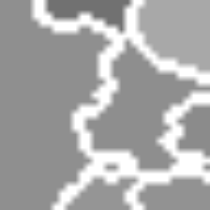
\includegraphics[width=.25\linewidth]{ipfs/ipfs-forest-unzipping-gui-b.png}}%
	\\
	\subfigure[Layer 3 before unzipping]{
\includegraphics[width=.25\linewidth]{ipfs/ipfs-forest-unzipping-gui-c.png}}%
	\hspace{8mm}%
	\subfigure[Select a node to unzip]{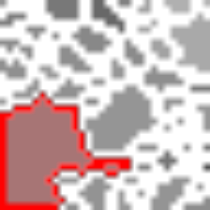
\includegraphics[width=.25\linewidth]{ipfs/ipfs-forest-unzipping-gui-d.png}}%
	\\
	\subfigure[Click the menu item]{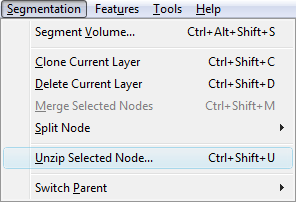
\includegraphics[width=.35\linewidth]{ipfs/ipfs-forest-unzipping-gui-e.png}}%
	\hspace{8mm}%
	\subfigure[Enter the target layer]{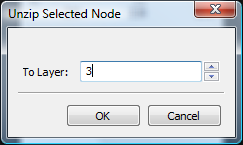
\includegraphics[width=.35\linewidth]{ipfs/ipfs-forest-unzipping-gui-f.png}}%
	\\
	\subfigure[Layer 2 after unzipping]{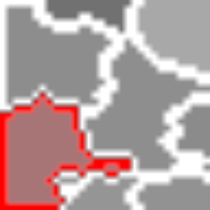
\includegraphics[width=.25\linewidth]{ipfs/ipfs-forest-unzipping-gui-g.png}}%
	\hspace{8mm}%
	\subfigure[Layer 3 after unzipping]{
\includegraphics[width=.25\linewidth]{ipfs/ipfs-forest-unzipping-gui-h.png}}%
\caption{The user interface for unzipping}
\label{fig:ipfs-forest-unzipping-gui}
\end{stusubfig}
%---

\paragraph{Precondition Checking}

The following preconditions must be checked for unzipping:

\begin{enumerate}

\item The node being unzipped must exist. (This can be checked in $O(1)$ time for the leaf layer, and $O(\log n_\ell)$ time for branch layer $\ell$.)
\item If $L$ is the layer containing the node being unzipped, and $H$ is the highest layer in the partition forest, then the index of the layer to which to unzip must be in the range $[L,H]$. (This can be trivially checked in $O(1)$ time.)

\end{enumerate}

\paragraph{Implementation}

Pseudo-code implementing the unzipping algorithm is shown in Listing~\ref{code:ipfs-forest-unzipnode}. As the algorithm progresses, we keep track of node chains that represent the strands being unzipped: these will be what is eventually returned as the result. In each iteration of the loop, we keep track of a `current' node, initially the input node. We determine the siblings of this node (defined to be the other children of its parent) and calculate their connected components. To these we add a singleton component containing the current node itself. We then split the parent of the current node into the specified components, update the aforementioned chains and repeat the process with the parent of the current node. The loop terminates when we reach the user-specified target layer.

The construction of the chains is the most interesting part of the algorithm. The way this works is most easily demonstrated by stepping through the unzipping example illustrated in Figure~\ref{fig:ipfs-forest-unzipping}. Initially, the array of chains is initialised with a singleton chain containing only the node being unzipped: in this case $(0,5)$.\footnote{This is an implementation trick that ensures that the chain leading up from the node being unzipped is the first chain in the array: this allows it to be easily identified by other algorithms that need ready access to it, such as \texttt{merge_nonsibling_nodes} (they would otherwise have to search through all the chains to find it). The final chain should not contain the actual node being unzipped (only the nodes above it), so in practice we remove it from the end of the chain again before returning.} During each iteration of the loop, each node resulting from that iteration's split node operation will either be used to augment an existing chain, or to add a new one: specifically, each existing chain is prepended with the parent of its head node, which is then removed from the set of nodes resulting from the split (it is guaranteed to be present because of the way the algorithm works); the remaining nodes resulting from the split are then used to create new singleton chains. In this example, the first iteration of the loop (in which \texttt{cur} = $(0,5)$, \texttt{parent} = $(1,2)$, \texttt{components} = $[\{2\}, \{5\}]$ and \texttt{result} = $\{(1,2), (1,5)\}$) results in \texttt{chains} being set to $[[(1,5), (0,5)], [(1,2)]]$. The second iteration (in which \texttt{cur} = $(1,5)$, \texttt{parent} = $(2,2)$, \texttt{components} = $[\{2\}, \{5\}, \{8\}]$ and \texttt{result} = $\{(2,2), (2,5), (2,8)\}$) results in \texttt{chains} being set to $[[(2,5), (1,5), (0,5)], [(2,2), (1,2)], [(2,8)]]$. The third iteration (in which \texttt{cur} = $(2,5)$, \texttt{parent} = $(3,2)$, \texttt{components} = $[\{2\}, \{5\}, \{8\}]$ and \texttt{result} = $\{(3,2), (3,5), (3,8)\}$) results in \texttt{chains} being set to $[[(3,5), (2,5), (1,5), (0,5)], [(3,2), (2,2), (1,2)], [(3,8), (2,8)]]$. Finally, $(0,5)$ is removed from the first chain, leaving the final chains to be returned by the algorithm as $[[(3,5), (2,5), (1,5)], [(3,2), (2,2), (1,2)], [(3,8), (2,8)]]$.

%---
\begin{stulisting}[p]
\caption{Forest : Unzipping : Implementation}
\label{code:ipfs-forest-unzipnode}
\lstinputlisting[style=Default]{ipfs/ipfs-forest-unzipnode.lst}
\end{stulisting}
%---

\paragraph{Complexity Analysis}

TODO

\afterpage{\clearpage}
\newpage

%~~~~~~~~~~~~~~~~~~~~~~~~~~~~~~~~~~~~~~~~~~~~~~~~
\subsubsection{Zipping}
%~~~~~~~~~~~~~~~~~~~~~~~~~~~~~~~~~~~~~~~~~~~~~~~~

\paragraph{Description}

A set of node chains (see the description of unzipping for a definition) that all start in the same layer can be zipped together, an operation that is effectively a multi-layer sibling node merge. When performed on the results of an unzip, this effectively undoes that operation. The zipping algorithm takes as input $k$ chains $[n_{1h},\ldots,n_{1\ell_1}], \ldots, [n_{kh},\ldots,n_{k\ell_k}]$ and returns a pair consisting of a node and a layer index, namely the parameters that we would need to pass to \texttt{unzip_node} in order to undo the operation. See Figure~\ref{fig:ipfs-forest-zipping} for an example.

%---
\begin{stusubfig}{p}
	\subfigure[Initial hierarchy]{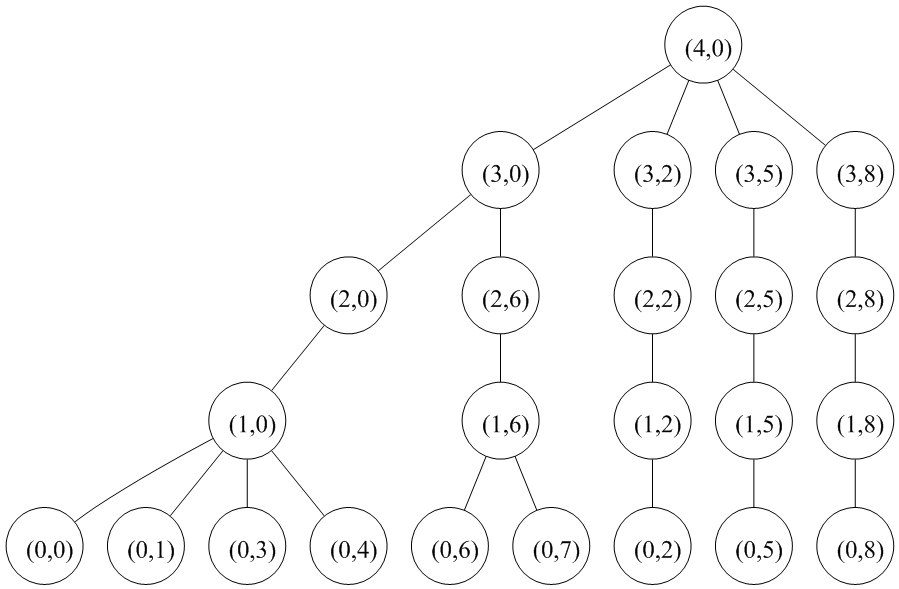
\includegraphics[width=.43\linewidth]{ipfs/ipfs-forest-zipping-a-hierarchy.png}}%
	\hspace{8mm}%
	\subfigure[After merging layer $3$ nodes]{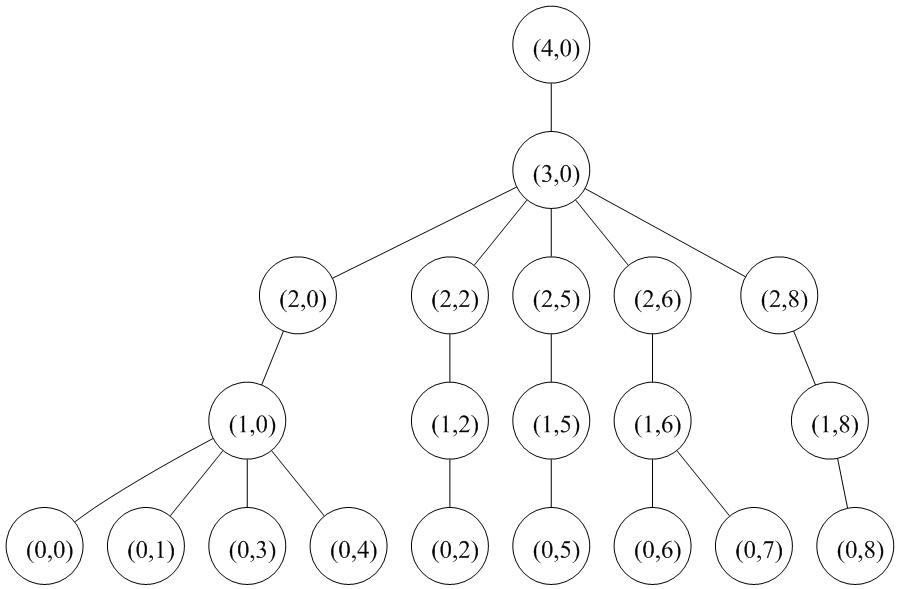
\includegraphics[width=.43\linewidth]{ipfs/ipfs-forest-zipping-b-hierarchy.png}}%
	\\
	\subfigure[After merging layer $2$ nodes]{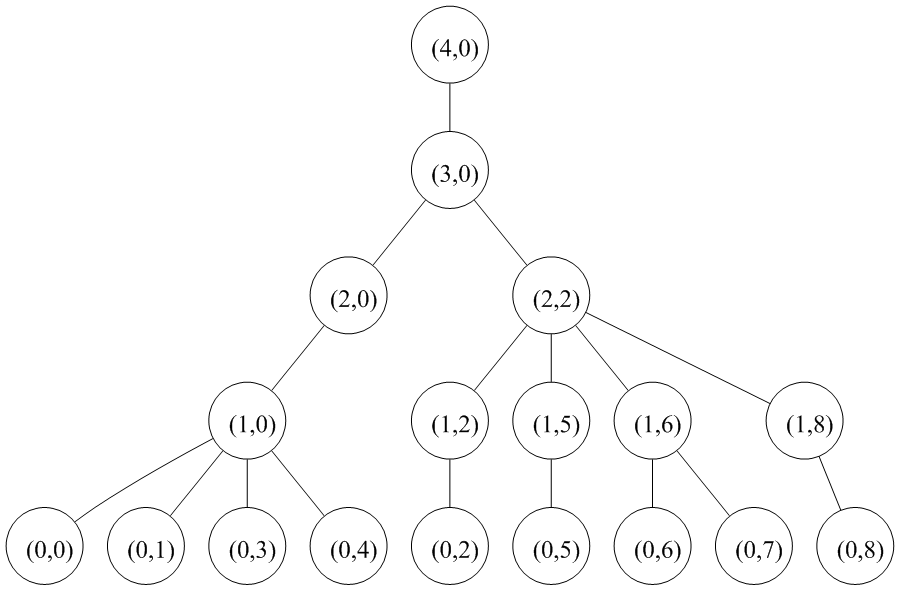
\includegraphics[width=.43\linewidth]{ipfs/ipfs-forest-zipping-c-hierarchy.png}}%
	\hspace{8mm}%
	\subfigure[After merging layer $1$ nodes]{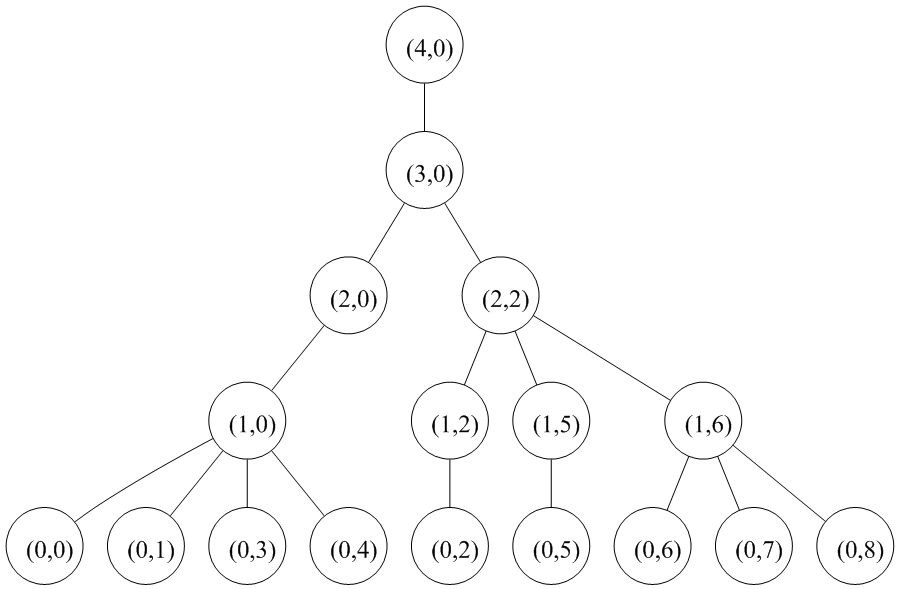
\includegraphics[width=.43\linewidth]{ipfs/ipfs-forest-zipping-d-hierarchy.png}}%
	\\
	\subfigure[Initial layer $1$ graph]{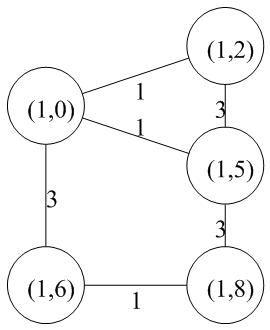
\includegraphics[width=.24\linewidth,height=.26\linewidth]{ipfs/ipfs-forest-zipping-a-graph1.png}}%
	\hspace{8mm}%
	\subfigure[Initial layer $2$ graph]{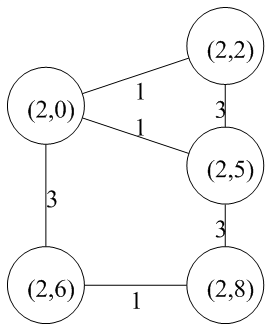
\includegraphics[width=.24\linewidth,height=.26\linewidth]{ipfs/ipfs-forest-zipping-a-graph2.png}}%
	\hspace{8mm}%
	\subfigure[Initial layer $3$ graph]{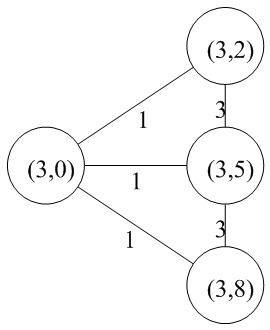
\includegraphics[width=.24\linewidth,height=.26\linewidth]{ipfs/ipfs-forest-zipping-a-graph3.png}}%
	\\
	\subfigure[Resulting layer $1$ graph]{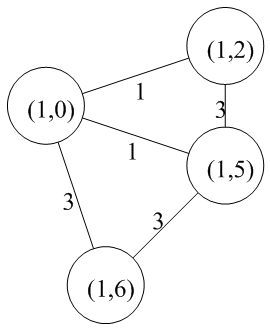
\includegraphics[width=.24\linewidth,height=.26\linewidth]{ipfs/ipfs-forest-zipping-d-graph1.png}}%
	\hspace{8mm}%
	\subfigure[Resulting layer $2$ graph]{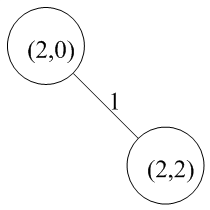
\includegraphics[width=.24\linewidth,height=.26\linewidth]{ipfs/ipfs-forest-zipping-c-graph2.png}}%
	\hspace{8mm}%
	\subfigure[Resulting layer $3$ graph]{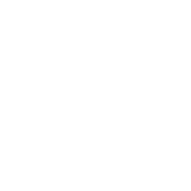
\includegraphics[width=.24\linewidth,height=.26\linewidth]{ipfs/ipfs-forest-zipping-b-graph3.png}}%
\caption{An example of zipping: zipping together the four chains $[(3,0), (2,6), (1,6)]$, $[(3,2), (2,2)]$, $[(3,5), (2,5)]$ and $[(3,8), (2,8), (1,8)]$}
\label{fig:ipfs-forest-zipping}
\end{stusubfig}
%---

\paragraph{C++ Method Interface}

\begin{lstlisting}[style=Prototype]
typedef deque<NodeID> Chain;
pair<NodeID,int> zip_chains(const vector<Chain>& chains);
\end{lstlisting}

\paragraph{User Interface for Image Analysis}

It doesn't make sense to expose zipping as part of the user interface, since the inputs it requires (node chains) are too cumbersome for the user to be asked to provide directly. More usable operations such as parent switching (described in the next section), that use zipping internally, should be exposed instead.

\paragraph{Precondition Checking}

The preconditions to be checked for zipping can be deduced from the preconditions required by the sibling node merges in terms of which it is implemented. There are at least two reasons for enforcing the preconditions at the zip level, rather than letting them be checked internally by the merges:

\begin{enumerate}

\item Zipping should be an \emph{atomic} forest operation -- that is, if the zip fails, the forest should be unchanged. Checking at the merge level can result in the zip being aborted after changes have been made to the forest, potentially leaving it in an inconsistent state.

\item Checking at the zip level is slightly more efficient -- in particular, we can exploit our knowledge about the sequence of merges to be performed in order to avoid checking in all but the top-most layer that the nodes to be merged are siblings.

\end{enumerate}

\noindent The following checks are thus necessary (see Listing~\ref{code:ipfs-forest-zipchains} for pseudo-code):

\begin{enumerate}

\item There must be chains to zip. (This can be trivially checked in $O(1)$ time.)
\item Each chain must be non-empty and consist only of valid nodes (TODO).
\item No chain must extend down as far as the leaf layer of the forest -- this guarantees that we will not be trying to merge leaf layer nodes.
\item The highest nodes in the chains must be siblings of each other. Note that there is no need to check that other corresponding nodes in the chains are siblings, as merging their parents in the previous iteration of the loop will automatically guarantee that they share the same parent.
\item The sets of nodes to be merged in each layer must be connected.

\end{enumerate}

\paragraph{Implementation}

Pseudo-code for the zipping algorithm is shown in Listing~\ref{code:ipfs-forest-zipchains}. The actual implementation is entirely straightforward (all the real work is in checking the preconditions). We start by determining the high and low layers of the chains. All the chains share the same high layer, so it suffices to take the high layer of the first chain in the array. The low layer is determined by a simple minimum element operation on the low layers of each of the individual chains. For each of the layers, from the top down, the relevant nodes are then extracted from the chains and merged using sibling node merging (note that there is no need to re-check the preconditions for each merge).

%---
\begin{stulisting}[p]
\caption{Forest : Zipping : Implementation}
\label{code:ipfs-forest-zipchains}
\lstinputlisting[style=Default]{ipfs/ipfs-forest-zipchains.lst}
\end{stulisting}
%---

\paragraph{Complexity Analysis}

TODO

\afterpage{\clearpage}
\newpage

%################################################
\subsection{Higher-Level Algorithms}
%################################################

Having discussed unzipping and zipping in the previous section, we are now in a position to implement two higher-level partition forest algorithms that are of great practical use. The first of these is the previously-mentioned merging operation that allows the user to merge nodes based on their adjacency in their forest layer (i.e.~in an imaging context, their spatial adjacency within the image) rather than whether or not they share a common forest parent. As observed earlier, this is the `intuitive' merging operation that the user wants to perform on forest nodes (see e.g.~Figure~\ref{fig:ipfs-forest-nonsiblingnodemerging-motivation}), but it is a difficult operation to implement without the machinery provided by the zipping algorithms.

The second higher-level algorithm that we can now implement is parent switching, the problem tackled in a more constrained manner by Peter Nacken in \cite{nacken95}. This operation mutates the forest so as to move a node from being the child of one parent to the child of another parent. As discussed in \S\ref{sec:background-partitionhierarchies}, there are two cases when this is problematic: (1) when the node is not adjacent to its new parent and (2) when moving the node would divide its old parent. Nacken's approach prevents nodes being moved in either of these two cases. There is clearly nothing that can be done about case (1) -- if the node is not adjacent to its new parent, then it can never be combined with the new parent's children to form a valid node. However, we will see that it is possible to use the zipping algorithms described here to develop a less constrained version of parent switching that still works in case (2) situations. (It should nevertheless be noted that Nacken's original analysis is entirely correct: it is not possible to switch the parent of a node in case (2) whilst keeping the old parent intact. The approach which I will describe circumvents this problem by allowing the old parent to be fragmented by the switch operation.)

\newpage

%~~~~~~~~~~~~~~~~~~~~~~~~~~~~~~~~~~~~~~~~~~~~~~~~
\subsubsection{Non-Sibling Node Merging}
%~~~~~~~~~~~~~~~~~~~~~~~~~~~~~~~~~~~~~~~~~~~~~~~~

\paragraph{Description}

A set of arbitrary nodes in any layer of the hierarchy other than the lowest can be divided into its connected components, each of which can then be merged. Since each component is connected, the result of each merge represents a valid object. From the user's perspective, this is a far more intuitive merge operation than sibling node merging: they simply have to indicate a set of nodes in a particular layer, and these are then merged into as few connected components as possible, based on their adjacency in the layer's graph. There is no requirement that the selected nodes are connected, or that they share a common parent (thus the user is freed from having to think about the structure of the forest when performing a merge). The algorithm takes as input the set of nodes to be merged, and returns the set of nodes resulting from merging each of the input's connected components (i.e.~there is one output node for each connected component of the input). An example is shown in Figure~\ref{fig:ipfs-forest-nonsiblingnodemerging}.

%---
\begin{stusubfig}{p}
	\subfigure[Initial hierarchy]{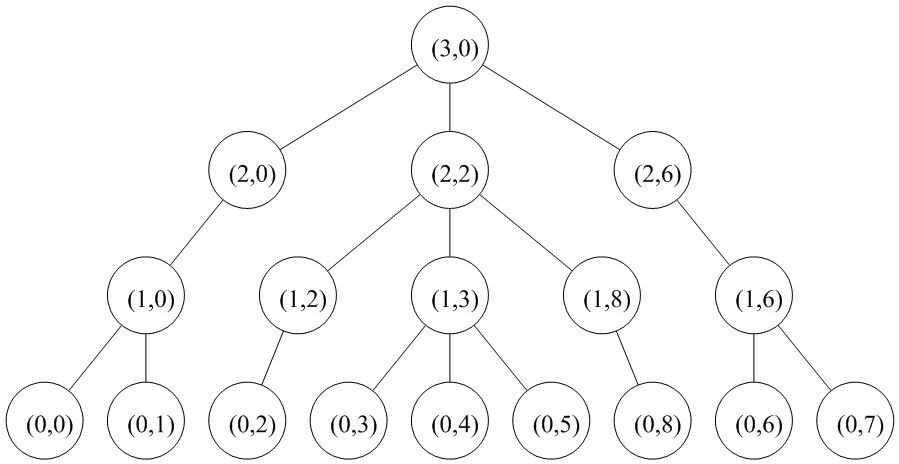
\includegraphics[width=.45\linewidth]{ipfs/ipfs-forest-nonsiblingnodemerging-a-hierarchy.png}}%
	\hspace{8mm}%
	\subfigure[After unzipping $(1,0)$ and $(1,2)$ to layer $2$]{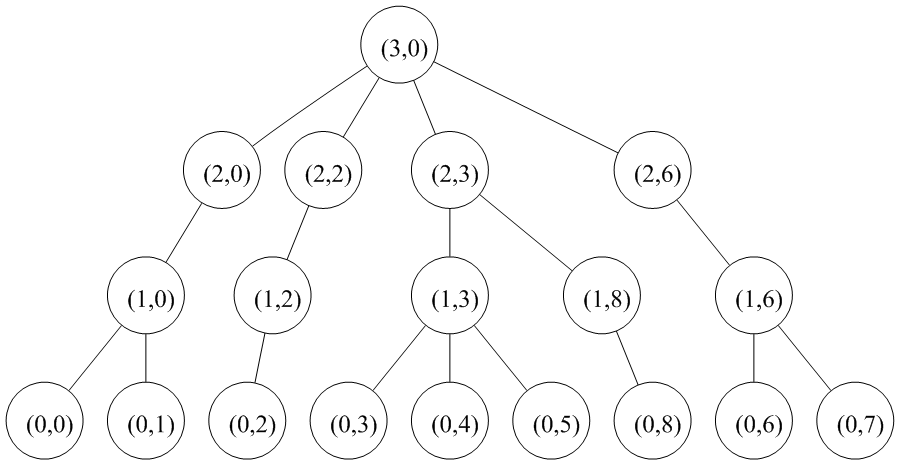
\includegraphics[width=.45\linewidth]{ipfs/ipfs-forest-nonsiblingnodemerging-c-hierarchy.png}}%
	\\
	\subfigure[{After zipping $[(2,0), (1,0)]$ and $[(2,2), (1,2)]$}]{\includegraphics[width=.45\linewidth]{ipfs/ipfs-forest-nonsiblingnodemerging-d-hierarchy.png}}%
	\hspace{8mm}%
	\subfigure[After unzipping $(1,6)$ and $(1,8)$ to layer $2$]{\includegraphics[width=.45\linewidth]{ipfs/ipfs-forest-nonsiblingnodemerging-f-hierarchy.png}}%
	\\
	\subfigure[{After zipping $[(2,6), (1,6)]$ and $[(2,8), (1,8)]$}]{\includegraphics[width=.45\linewidth]{ipfs/ipfs-forest-nonsiblingnodemerging-g-hierarchy.png}}%
\caption{An example of non-sibling node merging: merging nodes $(1,0)$, $(1,2)$, $(1,6)$ and $(1,8)$}
\label{fig:ipfs-forest-nonsiblingnodemerging}
\end{stusubfig}
%---

\paragraph{C++ Method Interface}

\begin{lstlisting}[style=Prototype]
set<NodeID> merge_nonsibling_nodes(const set<NodeID>& nodes);
\end{lstlisting}

\paragraph{User Interface for Image Analysis}

The user interface for non-sibling node merging is very simple, as illustrated in Figure~\ref{fig:ipfs-forest-nonsiblingnodemerging-gui}. The user selects some nodes, then clicks a menu item to merge them.

%---
\begin{stusubfig}{p}
	\subfigure[Layer 2 before merging]
	{\includegraphics[width=.3\linewidth]{ipfs/ipfs-forest-nonsiblingnodemerging-gui-a.png}}%
	%
	\hspace{8mm}%
	%
	\subfigure[Select the nodes to be merged]
	{\includegraphics[width=.3\linewidth]{ipfs/ipfs-forest-nonsiblingnodemerging-gui-b.png}}%
	%
	\\
	%
	\subfigure[Click the menu item]
	{\includegraphics[width=.4\linewidth]{ipfs/ipfs-forest-nonsiblingnodemerging-gui-c.png}}%
	%
	\hspace{8mm}%
	%
	\subfigure[Layer 2 after merging]
	{\includegraphics[width=.3\linewidth]{ipfs/ipfs-forest-nonsiblingnodemerging-gui-d.png}}%
\caption{The user interface for non-sibling node merging.}
\label{fig:ipfs-forest-nonsiblingnodemerging-gui}
\end{stusubfig}
%---

\paragraph{Precondition Checking}

The great advantage of non-sibling node merging over sibling node merging is that it has fewer preconditions; in fact, it owes its existence to the need to provide a less-constrained, more user-friendly merging algorithm for partition forest. It is therefore unsurprising that its preconditions are a strict subset of those of sibling node merging:

\begin{enumerate}

\item There must be more than one node to be merged. (This can be trivially checked in $O(1)$ time.)
\item None of the nodes must be in the lowest layer of the forest. (This can be checked in time linear in the number of nodes.)

\end{enumerate}

\paragraph{Implementation}

Pseudo-code to implement non-sibling node merging is shown in Listing~\ref{code:ipfs-forest-mergenonsiblingnodes}. The first step is to calculate the connected components of the input nodes: each connected component of size $> 1$ will be merged into one result node. To actually perform the merging for each connected component, we determine the common ancestor of the component's nodes. Each node is then unzipped to the layer below that containing the ancestor. In each case we keep track of the chain of nodes leading back down to the node being unzipped, appending the actual node being unzipped to the chain in each case (it would not otherwise be present). Finally, all of these chains are zipped together to merge the nodes in the connected component together.

For the example given in Figure~\ref{fig:ipfs-forest-nonsiblingnodemerging}, the connected components of the input nodes are $\{(1,0), (1,2)\}$ and $\{(1,6), (1,8)\}$. Both $(1,0)$ and $(1,2)$ are unzipped to layer $2$, the layer below their common ancestor $(3,0)$. The strands thus created are then zipped together, resulting in $(1,0)$ and $(1,2)$ being merged in layer $1$. An analogous process is used to merge $(1,6)$ and $(1,8)$.

%---
\begin{stulisting}[p]
\caption{Forest : Non-Sibling Node Merging : Implementation}
\label{code:ipfs-forest-mergenonsiblingnodes}
\lstinputlisting[style=Default]{ipfs/ipfs-forest-mergenonsiblingnodes.lst}
\end{stulisting}
%---

\paragraph{Complexity Analysis}

TODO

\afterpage{\clearpage}
\newpage

%~~~~~~~~~~~~~~~~~~~~~~~~~~~~~~~~~~~~~~~~~~~~~~~~
\subsubsection{Parent Switching}
%~~~~~~~~~~~~~~~~~~~~~~~~~~~~~~~~~~~~~~~~~~~~~~~~

\paragraph{Description}

A node in any layer of the hierarchy except the highest can be moved from being the child of its parent node to being the child of another node in the layer above, provided that it is adjacent to at least one child of its new parent. It is possible that moving the node may cause some of its old ancestors to become disconnected. If this happens, what remains of each old ancestor is split into its connected components. The algorithm takes as input the node to be moved and the index of its new parent node in the layer above. See Figure~\ref{fig:ipfs-forest-parentswitch} for an example.

%---
\begin{stusubfig}{p}
	\subfigure[The initial hierarchy]{\includegraphics[width=.5\linewidth]{ipfs/ipfs-forest-parentswitch-a-hierarchy.png}}%
	\hspace{4mm}%
	\subfigure[Layer $1$ graph]{\includegraphics[width=.2\linewidth]{ipfs/ipfs-forest-parentswitch-a-graph1.png}}%
	\hspace{4mm}%
	\subfigure[Layer $2$ graph]{\includegraphics[width=.2\linewidth]{ipfs/ipfs-forest-parentswitch-a-graph2.png}}%
	\\
	\subfigure[After unzipping $(0,4)$ to layer $2$]{\includegraphics[width=.5\linewidth]{ipfs/ipfs-forest-parentswitch-b-hierarchy.png}}%
	\hspace{4mm}%
	\subfigure[Layer $1$ graph]{\includegraphics[width=.2\linewidth]{ipfs/ipfs-forest-parentswitch-b-graph1.png}}%
	\hspace{4mm}%
	\subfigure[Layer $2$ graph]{\includegraphics[width=.2\linewidth]{ipfs/ipfs-forest-parentswitch-b-graph2.png}}%
	\\
	\subfigure[{After zipping $[(2,0), (1,0)]$ with $[(2,4), (1,4)]$}]{\includegraphics[width=.5\linewidth]{ipfs/ipfs-forest-parentswitch-c-hierarchy.png}}%
	\hspace{4mm}%
	\subfigure[Layer $1$ graph]{\includegraphics[width=.2\linewidth]{ipfs/ipfs-forest-parentswitch-c-graph1.png}}%
	\hspace{4mm}%
	\subfigure[Layer $2$ graph]{\includegraphics[width=.2\linewidth]{ipfs/ipfs-forest-parentswitch-c-graph2.png}}%
\caption{An example of parent switching: switching $(0,4)$'s parent to $(1,0)$}
\label{fig:ipfs-forest-parentswitch}
\end{stusubfig}
%---

\paragraph{C++ Method Interface}

\begin{lstlisting}[style=Prototype]
void parent_switch(const NodeID& node, int newParent);
\end{lstlisting}

\paragraph{User Interface for Image Analysis}

Like the user interface for node splitting, the interface for parent switching requires multiple steps (see Figure~\ref{fig:ipfs-forest-parentswitch-gui}). The user first selects the node whose parent is to be changed (the child in the switch operation) and marks it using a menu item. This causes the viewed layer to be changed to the layer above and its potential new parents to be highlighted (the potential new parents are the nodes in the layer above that have a child adjacent to the node being switched, excluding the node's current parent). The user selects one of these as the new parent and marks it using another menu item, thus effectuating the switch.

%---
\begin{stusubfig}{p}
	\subfigure[Layer 1 before parent switching]
	{\includegraphics[width=.25\linewidth]{ipfs/ipfs-forest-parentswitch-gui-a.png}}%
	%
	\hspace{8mm}%
	%
	\subfigure[Layer 2 before parent switching]
	{\includegraphics[width=.25\linewidth]{ipfs/ipfs-forest-parentswitch-gui-b.png}}%
	%
	\\
	%
	\subfigure[Select the child of the switch]
	{\includegraphics[width=.25\linewidth]{ipfs/ipfs-forest-parentswitch-gui-c.png}}%
	%
	\hspace{8mm}%
	%
	\subfigure[Mark it using the menu item]
	{\includegraphics[width=.45\linewidth]{ipfs/ipfs-forest-parentswitch-gui-d.png}}%
	%
	\\
	%
	\subfigure[Potential new parents are highlighted in green]
	{\includegraphics[width=.25\linewidth]{ipfs/ipfs-forest-parentswitch-gui-e.png}}%
	%
	\hspace{8mm}%
	%
	\subfigure[Select a new parent]
	{\includegraphics[width=.25\linewidth]{ipfs/ipfs-forest-parentswitch-gui-f.png}}%
	%
	\\
	%
	\subfigure[Perform the switch using the menu item]
	{\includegraphics[width=.45\linewidth]{ipfs/ipfs-forest-parentswitch-gui-g.png}}%
	%
	\hspace{8mm}%
	%
	\subfigure[Layer 2 after the switch]
	{\includegraphics[width=.25\linewidth]{ipfs/ipfs-forest-parentswitch-gui-h.png}}%
\caption{The user interface for parent switching.}
\label{fig:ipfs-forest-parentswitch-gui}
\end{stusubfig}
%---

\paragraph{Precondition Checking}

There are three preconditions that must be checked for parent switching (see Listing~\ref{code:ipfs-forest-parentswitch} for pseudo-code):

\begin{enumerate}

\item The node being moved must exist. (TODO)
\item The proposed new parent must exist.
\item The node must be adjacent to at least one child of its proposed new parent.

\end{enumerate}

\paragraph{Implementation}

Pseudo-code to implement parent switching is shown in Listing~\ref{code:ipfs-forest-parentswitch}. The first step is to determine the common ancestor of the current and new parents of the node being moved (in the example, this would be the common ancestor of $(1,3)$ and $(1,0)$, namely $(3,0)$). In the process of doing so, we make sure to keep track of the chain of nodes leading down from the common ancestor (non-inclusive) to the new parent (in the example, this would be $[(2,0), (1,0)]$). The node being moved is then unzipped to the layer below the common ancestor, and its chain leading down from the common ancestor (non-inclusive) must then be zipped to the chain leading down the new parent. This completes the move.

%---
\begin{stulisting}[p]
\caption{Forest : Parent Switching : Implementation}
\label{code:ipfs-forest-parentswitch}
\lstinputlisting[style=Default]{ipfs/ipfs-forest-parentswitch.lst}
\end{stulisting}
%---

\paragraph{Complexity Analysis}

TODO

\afterpage{\clearpage}
\newpage

%################################################
\subsection{Summary}
%################################################

TODO: Summarise the algorithms and their complexities

\newpage

%##################################################################################################
\section{Partition Forest Selections}
\label{sec:ipfs-selections}
%##################################################################################################

In order for users to interact with partition forests, they must be able to select parts of them with which to work (we have seen examples of this when describing the mutating algorithms in the previous section). It is in principle easy enough to manage the selection of individual nodes -- by maintaining a set of currently selected nodes, for instance -- and this suffices when selecting nodes in a single layer of the forest. However, in an interactive system, there are times when it is desirable to be able to manage the selection of nodes in multiple layers of the hierarchy -- for instance, the user may wish to select a large region in one layer and then refine it by deselecting some of its children in the layer below (see Figure~\ref{?}). For this, the simplistic approach is insufficient, because it ignores the forest's hierarchical structure. In particular, with this scheme, the selection of a node in one layer does not imply that its children in the layer below are also selected -- so it is impossible to deselect some of them as desired. Furthermore, the simple approach allows the simultaneous selection of a node and some (but not all) of its descendants, making the selection system unintuitive and hard to use (if the user chooses to deselect a node, it is rather confusing if some of it remains selected afterwards).

For this reason, it is necessary to introduce a more sophisticated approach to partition forest selection that takes hierarchy into account. In what follows, I therefore describe a novel data structure and algorithms for partition forest selection (expanding on work originally presented in \cite{gvcispa09}) that treat the selection of a node as implicitly selecting the subtree of which it is the root, without an implementation having to explicitly maintain the set of selected nodes in the subtree (which would be prohibitively expensive). This solves both of the problems described above. I also describe how partition forest selections should be updated in response to changes to the partition forest to which they refer (implemented in practice using the standard \emph{observer} pattern \cite{gamma95}) -- this is clearly crucially important when implementing an interactive system, especially since the selections could otherwise end up referring to forest nodes that no longer exist.

%################################################
\subsection{Data Structure}
%################################################

The partition forest selection data structure should contain an array of sets of node indices, one per forest layer, and some type of pointer to the partition forest to which it corresponds.\footnote{The actual code also contains a pointer to the application's command manager and a `composite listener' to allow observers to listen to changes in the selection, but these are implementation details.} In C++, this can be implemented as follows (noting that \texttt{shared_ptr} is a kind of reference-counted smart pointer):

\begin{lstlisting}[style=Default,language=C++]
template <typename LeafLayer, typename BranchLayer>
class PartitionForestSelection
{
	typedef set<int> Layer;

	vector<Layer> nodes;
	shared_ptr<PartitionForest<LeafLayer,BranchLayer>> forest;

	//...
};
\end{lstlisting}

The \texttt{nodes} data member will contain nodes that represent the selection, but many representations are possible. Specifically, we note that the selection of a set of nodes in multiple layers of the forest corresponds to the selection of a set of pixels (or voxels, in 3D) in the forest's leaf layer (see Figure~\ref{?}). This is a many-to-one relationship: there are many node selections that correspond to the same pixel selection (it is possible to define an equivalence relation that makes all the node selections corresponding to the selection of a particular set of pixels equivalent). However, we are only interested in non-redundant representations of the pixel selection: more precisely, in sets of nodes that partition the pixel selection (they cover all the pixels and do not overlap). As Figure~\ref{?} illustrates, there are still many sets of nodes that would satisfy this criterion for a given pixel selection, but of the sets whose size is the smallest, there is always one unique set whose nodes are in the highest forest layers possible. We describe this as the \emph{hierarchical node representation} of a given pixel selection $S$, and denote it $\textbf{HNR}(S)$. This is an ideal representation for partition forest selections, because it contains all the information necessary and in the most compact form possible. We thus maintain precisely the nodes in $\textbf{HNR}(S)$ in the \texttt{nodes} data member, for whatever $S$ happens to be selected at the time.

%################################################
\subsection{Overview of Algorithms}
%################################################

Having defined the partition forest selection data structure, and in particular the way in which selections are represented, we next turn to the algorithms that should be implemented for partition forest selections. These can be divided into three groups:

\begin{enumerate}

\item The \textbf{core} algorithms implement basic functionality: the \emph{node selection} and \emph{node deselection} algorithms allow the selection and deselection of individual nodes, respectively, whilst the \emph{view at layer} algorithm allows the selection to be viewed at a specific forest layer (all nodes in higher layers are replaced with their descendants in the chosen layer).

\item The \textbf{undo} algorithms, \emph{undo modification} and \emph{redo modification}, allow changes to the selection to be undone/redone.

\item Finally, the \textbf{listening} algorithms listen to the partition forest to which the selection corresponds, and update the selection in response to any changes. The selection needs to change in response to each of the core partition forest algorithms: layer cloning, layer deletion/undeletion, sibling node merging and node splitting. It should be noted that because the remaining partition forest algorithms were implemented in terms of the core algorithms, there is no need for additional algorithms that update the selection in response to e.g.~unzipping or parent switching. This is a major advantage of the implementation technique chosen.

\end{enumerate}

\noindent The \textbf{binary set} algorithms \emph{union selections} and \emph{subtract selections} also need to be implemented if selections are to be compared for validation purposes, but these can be trivially implemented in terms of \emph{node selection} and \emph{node deselection} (see Appendix~\ref{chap:appendixpf}).

%################################################
\subsection{Core Algorithms}
%################################################

%~~~~~~~~~~~~~~~~~~~~~~~~~~~~~~~~~~~~~~~~~~~~~~~~
\subsubsection{Node Selection}
%~~~~~~~~~~~~~~~~~~~~~~~~~~~~~~~~~~~~~~~~~~~~~~~~

\paragraph{Description}

Any node in the partition forest can be added to the selection. This has the effect of ensuring that the entire subtree below the input node in the forest is selected. The algorithm takes a single node as input, and returns the modification this caused to the selection. A \emph{selection modification} is a pair of node sets -- \texttt{(erased, inserted)} -- containing the specific nodes that were erased from/inserted into the selection representation. It can be passed to the \emph{undo modification} algorithm to undo the changes made to the selection.

\paragraph{C++ Method Interface}

\begin{lstlisting}[style=Prototype]
Modification select_node(const NodeID& node);
\end{lstlisting}

\paragraph{Implementation}

As I originally discussed in \cite{gvcispa09}, there are four cases to deal with when adding a node to the selection:

\begin{enumerate}

\item The node itself is already in the representation (that is, it is itself contained in the \texttt{nodes} data member).
\item An ancestor of the node is already in the representation.
\item One or more descendants of the node is already in the representation.
\item Neither the node nor any of its ancestors or descendants is already in the representation.

\end{enumerate}

\noindent In the first two cases, nothing needs to be done: since either the input node or one of its ancestors is in the representation, all the nodes in the subtree below the input node are already implicitly selected. The third and fourth cases require more work. In the third case, all descendants of the node must first be removed from the representation (and thus added to the \texttt{erased} component of the selection modification). Then, in both cases, the input node itself must be added to the representation (and thus to the \texttt{inserted} component of the selection modification). Finally, a process of \emph{consolidation} must take place to ensure that the selection is still represented using the hierarchical representation we defined: this involves replacing any node whose children are all part of the representation with the node itself, until this is no longer possible. In practice, when consolidating after selecting a node, we only need to worry about nodes that are ancestors of the input node -- we thus recursively consolidate upwards from the parent of the input node, terminating when either one of the children of the node currently being examined is not part of the representation, or when we reach the top of the forest. An example illustrating this process is shown in Figure~\ref{fig:ipfs-selection-nodeselection}. After the initial insertion, the selection modification is $(\emptyset,\{(0,3)\})$. As the ancestors are consolidated, it then changes to $(\{(0,2), (0,4)\}, \{(1,2)\})$, $(\{(0,2), (0,4), (1,0)\}, \{(2,0)\})$ and finally $(\{(0,2), (0,4), (1,0), (2,5)\}, \{(3,0)\})$. Pseudo-code for the main algorithm is shown in Listing~\ref{code:ipfs-selection-selectnodeimpl}; pseudo-code for the consolidation process can be found in Appendix~\ref{chap:appendixpf}.

TODO: Complexity analysis

%---
\begin{stusubfig}{p}
	\subfigure[The initial selection]{\includegraphics[width=.3\linewidth]{ipfs/ipfs-selection-nodeselection-a-hierarchy.png}}%
	\hspace{4mm}%
	\subfigure[After adding $(0,3)$]{\includegraphics[width=.3\linewidth]{ipfs/ipfs-selection-nodeselection-b-hierarchy.png}}%
	\hspace{4mm}%
	\subfigure[After consolidating $(1,2)$]{\includegraphics[width=.3\linewidth]{ipfs/ipfs-selection-nodeselection-c-hierarchy.png}}%
	\\
	\subfigure[After consolidating $(2,0)$]{\includegraphics[width=.3\linewidth]{ipfs/ipfs-selection-nodeselection-d-hierarchy.png}}%
	\hspace{4mm}%
	\subfigure[After consolidating $(3,0)$]{\includegraphics[width=.3\linewidth]{ipfs/ipfs-selection-nodeselection-e-hierarchy.png}}%
\caption{An example of node selection: adding $(0,3)$ to the selection}
\label{fig:ipfs-selection-nodeselection}
\end{stusubfig}
%---

%---
\begin{stulisting}[p]
\caption{Forest Selection : Node Selection : Implementation}
\label{code:ipfs-selection-selectnodeimpl}
\lstinputlisting[style=Default]{ipfs/ipfs-selection-selectnodeimpl.lst}
\end{stulisting}
%---

\afterpage{\clearpage}
\newpage

%~~~~~~~~~~~~~~~~~~~~~~~~~~~~~~~~~~~~~~~~~~~~~~~~
\subsubsection{Node Deselection}
%~~~~~~~~~~~~~~~~~~~~~~~~~~~~~~~~~~~~~~~~~~~~~~~~

\paragraph{Description}

Any node in the partition forest can be removed from the selection. This has the effect of ensuring that the entire subtree below the input node in the forest is deselected. The algorithm takes a single node as input, and returns the modification this caused to the selection.

\paragraph{C++ Method Interface}

\begin{lstlisting}[style=Prototype]
Modification deselect_node(const NodeID& node);
\end{lstlisting}

\paragraph{Implementation}

As with node selection, there are the same four cases to deal with when removing a node from the selection:

\begin{enumerate}

\item The node itself is in the representation.
\item An ancestor of the node is in the representation.
\item One or more descendants of the node is in the representation.
\item Neither the node nor any of its ancestors or descendants is in the representation.

\end{enumerate}

\noindent Case $1$ is trivial: we can simply remove the node from the representation directly. Case $4$ is likewise trivial, as the selection does not even need to be modified. In Case $3$, it suffices to enumerate all the descendants of the node that are in the representation and remove them all.

The more interesting case is Case $2$, in which one of the node's ancestors is in the selection representation. In that case, we must find the \emph{trail} of nodes in the forest leading from the ancestor in question to the node itself (non-inclusive). We then replace all the nodes on this trail (from the ancestor downwards) with their children until the node we want to deselect is part of the representation, at which point we can simply remove it. An example of this process is shown in Figure~\ref{fig:ipfs-selection-nodedeselection}. In this case, the selected ancestor is $(3,0)$ and the trail is $[(3,0), (2,0), (1,2)]$. Each of the nodes on the trail is split in turn. Eventually, $(0,3)$ is in the representation, and can be removed. Pseudo-code for the main algorithm is shown in Listing~\ref{code:ipfs-selection-deselectnodeimpl}; pseudo-code for the subsidiary processes can be found in Appendix~\ref{chap:appendixpf}.

TODO: Complexity analysis

%---
\begin{stusubfig}{p}
	\subfigure[The initial selection]{\includegraphics[width=.3\linewidth]{ipfs/ipfs-selection-nodeselection-e-hierarchy.png}}%
	\hspace{4mm}%
	\subfigure[After splitting $(3,0)$]{\includegraphics[width=.3\linewidth]{ipfs/ipfs-selection-nodeselection-d-hierarchy.png}}%
	\hspace{4mm}%
	\subfigure[After splitting $(2,0)$]{\includegraphics[width=.3\linewidth]{ipfs/ipfs-selection-nodeselection-c-hierarchy.png}}%
	\\
	\subfigure[After splitting $(1,2)$]{\includegraphics[width=.3\linewidth]{ipfs/ipfs-selection-nodeselection-b-hierarchy.png}}%
	\hspace{4mm}%
	\subfigure[After removing $(0,3)$]{\includegraphics[width=.3\linewidth]{ipfs/ipfs-selection-nodeselection-a-hierarchy.png}}%
\caption{An example of node deselection: removing $(0,3)$ from the selection}
\label{fig:ipfs-selection-nodedeselection}
\end{stusubfig}
%---

%---
\begin{stulisting}[p]
\caption{Forest Selection : Node Deselection : Implementation}
\label{code:ipfs-selection-deselectnodeimpl}
\lstinputlisting[style=Default]{ipfs/ipfs-selection-deselectnodeimpl.lst}
\end{stulisting}
%---

\afterpage{\clearpage}
\newpage

%~~~~~~~~~~~~~~~~~~~~~~~~~~~~~~~~~~~~~~~~~~~~~~~~
\subsubsection{View At Layer}
%~~~~~~~~~~~~~~~~~~~~~~~~~~~~~~~~~~~~~~~~~~~~~~~~

\paragraph{Description}

In a number of situations (most notably when rendering the selected nodes in an interactive application), it is important to be able to view the selection representation from a specific layer of the forest. This has the effect of splitting any nodes in the representation that are in higher forest layers into their descendants in the specified layer. All nodes in the representation that are in the specified layer or below are unaffected.

A motivation for this operation is best illustrated by Figure~\ref{fig:ipfs-selection-viewatlayer-motivation}. In (a), the user has selected a node in layer $2$ of a forest. If they subsequently want to deselect a child of this node in layer $1$, they need to view the selection from the perspective of layer $1$ in order to see the nodes that they can deselect (shown in (b)). This is handled by the \emph{view at layer} algorithm described here.

%---
\begin{stusubfig}{p}
	\subfigure[Selecting a node in layer $2$]{\includegraphics[width=.3\linewidth]{ipfs/ipfs-selection-viewatlayer-motivation-a.png}}%
	\hspace{4mm}%
	\subfigure[Viewing it at layer $1$]{\includegraphics[width=.3\linewidth]{ipfs/ipfs-selection-viewatlayer-motivation-b.png}}%
\caption{The motivation for the view at layer algorithm}
\label{fig:ipfs-selection-viewatlayer-motivation}
\end{stusubfig}
%---

The theoretical algorithm takes as input the layer at which to view the selection representation, and returns a vector containing the selected nodes as viewed at that layer. In practice, however, the algorithm is actually implemented using iterators that allow the client to step through the nodes in the view, splitting higher-level nodes on demand. This makes it possible to avoid storing all the nodes in the view unnecessarily.

\paragraph{C++ Method Interface}

The theoretical interface is:

\begin{lstlisting}[style=Prototype]
vector<NodeID> view_at_layer(int layerIndex);
\end{lstlisting}

\noindent If the algorithm is implemented using iterators, however, the interface becomes:

\begin{lstlisting}[style=Prototype]
ViewNodeConstIterator view_at_layer_cbegin(int layerIndex);
ViewNodeConstIterator view_at_layer_cend(int layerIndex);
\end{lstlisting}

\paragraph{Implementation}

The non-iterator-based implementation of the algorithm is straightforward (see Listing~\ref{code:ipfs-selection-viewatlayer} for pseudo-code). The first loop iterates through all the layers strictly higher than the one specified and adds the descendants of the selected nodes in the specified layer to the vector of result nodes. The second loop then iterates through all the remaining layers and adds their selected nodes directly to the vector of result nodes. An example showing the results of viewing a selection at a particular layer is shown in Figure~\ref{fig:ipfs-selection-viewatlayer}.

Implementing an iterator-based version of the algorithm is only marginally more difficult (see Appendix~\ref{chap:appendixpf} for pseudo-code). The key is to first implement a normal iterator that iterates over all the nodes in the representation in order, starting with those in the highest layer. A viewing iterator can then be implemented relatively easily in terms of this.

TODO: Complexity analysis

%---
\begin{stusubfig}{p}
	\subfigure[The actual selection]{\includegraphics[width=.45\linewidth]{ipfs/ipfs-selection-viewatlayer-a-hierarchy.png}}%
	\hspace{4mm}%
	\subfigure[The selection viewed at layer $1$]{\includegraphics[width=.45\linewidth]{ipfs/ipfs-selection-viewatlayer-b-hierarchy.png}}%
\caption{An example of the view at layer algorithm}
\label{fig:ipfs-selection-viewatlayer}
\end{stusubfig}
%---

%---
\begin{stulisting}[p]
\caption{Forest Selection : View at Layer : Implementation}
\label{code:ipfs-selection-viewatlayer}
\lstinputlisting[style=Default]{ipfs/ipfs-selection-viewatlayer.lst}
\end{stulisting}
%---

\afterpage{\clearpage}
\newpage

%################################################
\subsection{Undo Algorithms}
%################################################

%~~~~~~~~~~~~~~~~~~~~~~~~~~~~~~~~~~~~~~~~~~~~~~~~
\subsubsection{Undo Modification}
%~~~~~~~~~~~~~~~~~~~~~~~~~~~~~~~~~~~~~~~~~~~~~~~~

As previously mentioned, the \emph{node selection} and \emph{node deselection} algorithms return selection modifications that can be used to undo their effects. The \emph{undo modification} algorithm reinserts nodes that were erased from the representation, and removes nodes that were inserted:

\begin{lstlisting}[style=Default]
function undo_modification
:	(modification : Modification) $\to \emptyset$

	for each n : NodeID $\in$ modification.erased_nodes()
		insert_node(n, null);
	for each n : NodeID $\in$ modification.inserted_nodes()
		erase_node(n, null);
	listeners.modification_undone(modification);
\end{lstlisting}

\noindent TODO: Complexity analysis

%~~~~~~~~~~~~~~~~~~~~~~~~~~~~~~~~~~~~~~~~~~~~~~~~
\subsubsection{Redo Modification}
%~~~~~~~~~~~~~~~~~~~~~~~~~~~~~~~~~~~~~~~~~~~~~~~~

Selection modifications that were undone by \emph{undo modification} can also be redone (there is no need to execute the original command a second time, which would involve recalculating the necessary nodes to erase/insert). The \emph{redo modification} algorithm re-erases any nodes in the \texttt{erased} set, and re-inserts any nodes in the \texttt{inserted} set:

\begin{lstlisting}[style=Default]
function redo_modification
:	(modification : Modification) $\to \emptyset$

	for each n : NodeID $\in$ modification.erased_nodes()
		erase_node(n, null);
	for each n : NodeID $\in$ modification.inserted_nodes()
		insert_node(n, null);
	listeners.modification_redone(modification);
\end{lstlisting}

\noindent TODO: Complexity analysis

\newpage

%################################################
\subsection{Listening Algorithms}
%################################################

%~~~~~~~~~~~~~~~~~~~~~~~~~~~~~~~~~~~~~~~~~~~~~~~~
\subsubsection{Layer Was Cloned}
%~~~~~~~~~~~~~~~~~~~~~~~~~~~~~~~~~~~~~~~~~~~~~~~~

\paragraph{Description}

When a layer in the forest is cloned, the selection representation must have an additional layer added to it, and any selected nodes in the cloned layer must be migrated to the layer above. For instance, if the node $(2,0)$ is in the representation, and layer $2$ is cloned, then an identical layer $3$ will be inserted above it. If that happens, the selections of $(2,0)$ and $(3,0)$ will be equivalent, except that $(3,0)$ is higher in the forest. We must thus replace $(2,0)$ with $(3,0)$ in the representation.

\paragraph{C++ Method Interface}

\begin{lstlisting}[style=Prototype]
void layer_was_cloned(int index);
\end{lstlisting}

\paragraph{Implementation}

Rather than inserting the new layer into the selection representation above the cloned layer, and then migrating any nodes upwards, the actual implementation instead inserts an empty layer into the representation below the cloned layer:

\begin{lstlisting}[style=Default]
function layer_was_cloned
:	(index : int) $\to \emptyset$

	// The desired effect is to insert a layer above the one specified and migrate
	// any selected nodes upwards to the new layer. This can be achieved most easily
	// by simply inserting an empty layer below the one being cloned, as here.
	var emptyLayer : SelectionLayer;
	insert_layer(index, emptyLayer);

	listeners.selection_changed();
\end{lstlisting}

\noindent This has the effect of pushing any selected nodes in the cloned layer upwards, without extra work being needed to handle them.

\newpage

%~~~~~~~~~~~~~~~~~~~~~~~~~~~~~~~~~~~~~~~~~~~~~~~~
\subsubsection{Layer Will Be Deleted / Layer Was Deleted}
%~~~~~~~~~~~~~~~~~~~~~~~~~~~~~~~~~~~~~~~~~~~~~~~~

\paragraph{Description}

When a layer is deleted from the forest, the selection must react by replacing any selected nodes in the deleted layer with their children in the layer below. To do this, it must be informed \emph{before} the layer is actually deleted (i.e.~while it can still query the forest for the children of the selected nodes). An example is shown in Figure~\ref{fig:ipfs-selection-layerwillbedeleted}.

%---
\begin{stusubfig}{p}
	\subfigure[Before deleting layer $3$]{\includegraphics[width=.6\linewidth]{ipfs/ipfs-selection-layerwillbedeleted-a-hierarchy.png}}%
	\hspace{4mm}%
	\subfigure[After deleting layer $3$]{\includegraphics[width=.6\linewidth]{ipfs/ipfs-selection-layerwillbedeleted-b-hierarchy.png}}%
\caption{An example of the layer will be deleted algorithm}
\label{fig:ipfs-selection-layerwillbedeleted}
\end{stusubfig}
%---

\paragraph{C++ Method Interfaces}

\begin{lstlisting}[style=Prototype]
void layer_will_be_deleted(int index);
void layer_was_deleted(int index);
\end{lstlisting}

\paragraph{Implementation}

The implementation is straightforward, as shown in Listing~\ref{code:ipfs-selection-layerwillbedeleted}. Each selected node in the layer to be deleted is first \emph{deconsolidated} (that is, it is replaced in the selection representation by its children in the layer below). The layer itself is then erased from the selection representation. Listeners are only informed after the layer has actually been deleted from the forest (not just the selection), because the forest and selection will temporarily have different numbers of layers until this has been done (as far as listeners are concerned, they must satisfy the invariant of having the same number of layers).

%---
\begin{stulisting}[p]
\caption{Forest Selection : Layer Will Be Deleted / Layer Was Deleted : Implementation}
\label{code:ipfs-selection-layerwillbedeleted}
\lstinputlisting[style=Default]{ipfs/ipfs-selection-layerwillbedeleted.lst}
\end{stulisting}
%---

\afterpage{\clearpage}
\newpage

%~~~~~~~~~~~~~~~~~~~~~~~~~~~~~~~~~~~~~~~~~~~~~~~~
\subsubsection{Layer Was Undeleted}
%~~~~~~~~~~~~~~~~~~~~~~~~~~~~~~~~~~~~~~~~~~~~~~~~

\paragraph{Description}

When a forest layer is undeleted, the selection must do the opposite of what it did when the layer was deleted: that is, after recreating the layer in the selection representation, it must \emph{consolidate} at least the nodes that were previously deconsolidated when the layer was deleted. It could certainly consolidate all the nodes in the newly recreated layer, but that would be wasteful; a better approach is to consolidate only the parents of the selected nodes in the layer below.

An example is shown in Figure~\ref{fig:ipfs-selection-layerwasundeleted}: the only nodes that actually need consolidating are those that were actually selected before the layer deletion (shown in red), but in practice the way the algorithm works means that we also consolidate nodes whose children are not all selected as well (shown in pink). Note that consolidating such nodes involves some redundant checks (as these nodes will not ultimately replace their children in the selection), but this is still far better than consolidating all the nodes in the layer being undeleted.

%---
\begin{stusubfig}{p}
	\subfigure[The original selection]{\includegraphics[width=.45\linewidth]{ipfs/ipfs-selection-layerwasundeleted-a-hierarchy.png}}%
	\\
	\subfigure[After deleting layer $2$]{\includegraphics[width=.45\linewidth]{ipfs/ipfs-selection-layerwasundeleted-b-hierarchy.png}}%
	\\
	\subfigure[Consolidating the nodes during undeletion]{\includegraphics[width=.45\linewidth]{ipfs/ipfs-selection-layerwasundeleted-c-hierarchy.png}}%
\caption{An example of the layer was undeleted algorithm}
\label{fig:ipfs-selection-layerwasundeleted}
\end{stusubfig}
%---

\paragraph{C++ Method Interface}

\begin{lstlisting}[style=Prototype]
void layer_was_undeleted(int index);
\end{lstlisting}

\paragraph{Implementation}

Pseudo-code to implement the algorithm is shown in Listing~\ref{code:ipfs-selection-layerwasundeleted}. First, an empty layer must be re-added to the selection representation in the appropriate place. Then, a set is constructed containing the parents of the selected nodes in the layer below that being undeleted. Finally, each of those parents is consolidated in turn.

TODO: Complexity analysis

%---
\begin{stulisting}[p]
\caption{Forest Selection : Layer Was Undeleted : Implementation}
\label{code:ipfs-selection-layerwasundeleted}
\lstinputlisting[style=Default]{ipfs/ipfs-selection-layerwasundeleted.lst}
\end{stulisting}
%---

\afterpage{\clearpage}
\newpage

%~~~~~~~~~~~~~~~~~~~~~~~~~~~~~~~~~~~~~~~~~~~~~~~~
\subsubsection{Nodes Will Be Merged / Nodes Were Merged}
%~~~~~~~~~~~~~~~~~~~~~~~~~~~~~~~~~~~~~~~~~~~~~~~~

\paragraph{Description}

When sibling nodes in the forest are merged, the selection needs to be informed both before and after it happens. If selected nodes are about to be merged, then they must be deconsolidated, as they will cease to exist once the merge takes place. After the merge, the result node must then be consolidated, as it is possible that all the nodes being merged were selected prior to the merge happening. An example is shown in Figure~\ref{fig:ipfs-selection-nodeswillbemerged}. In (b), the selection is informed that $(1,0)$ and $(1,1)$ are about to be merged, so it deconsolidates $(1,0)$ (as that is currently selected). In (c), the two nodes are then merged. In (d), $(1,0)$ is consolidated, but is not re-selected because $(0,1)$ is not part of the selection. The same thing happens when merging $(1,2)$ and $(1,3)$, except that the consolidation step in (g) replaces $(0,2)$ and $(0,3)$ with $(1,2)$ after the merge, since all of the latter's children are selected.

%---
\begin{stusubfig}{p}
	\subfigure[The original selection]{\includegraphics[width=.3\linewidth]{ipfs/ipfs-selection-nodeswillbemerged-a-hierarchy.png}}%
	\hspace{4mm}%
	\subfigure[$(1,0)$ and $(1,1)$ will merge]{\includegraphics[width=.3\linewidth]{ipfs/ipfs-selection-nodeswillbemerged-b-hierarchy.png}}%
	\hspace{4mm}%
	\subfigure[$(1,0)$ and $(1,1)$ merge]{\includegraphics[width=.3\linewidth]{ipfs/ipfs-selection-nodeswillbemerged-c-hierarchy.png}}%
	\hspace{4mm}%
	\subfigure[$(1,0)$ and $(1,1)$ were merged]{\includegraphics[width=.3\linewidth]{ipfs/ipfs-selection-nodeswillbemerged-d-hierarchy.png}}%
	\hspace{4mm}%
	\subfigure[$(1,2)$ and $(1,3)$ will merge]{\includegraphics[width=.3\linewidth]{ipfs/ipfs-selection-nodeswillbemerged-e-hierarchy.png}}%
	\hspace{4mm}%
	\subfigure[$(1,2)$ and $(1,3)$ merge]{\includegraphics[width=.3\linewidth]{ipfs/ipfs-selection-nodeswillbemerged-f-hierarchy.png}}%
	\hspace{4mm}%
	\subfigure[$(1,2)$ and $(1,3)$ were merged]{\includegraphics[width=.3\linewidth]{ipfs/ipfs-selection-nodeswillbemerged-g-hierarchy.png}}%
\caption{An example of the nodes will be merged / nodes were merged algorithms}
\label{fig:ipfs-selection-nodeswillbemerged}
\end{stusubfig}
%---

\paragraph{C++ Method Interface}

\begin{lstlisting}[style=Prototype]
void nodes_will_be_merged(const set<NodeID>& nodes);
void nodes_were_merged(const set<NodeID>& nodes,
                       const NodeID& result);
\end{lstlisting}

\paragraph{Implementation}

The implementation, as shown in the pseudo-code in Listing~\ref{code:ipfs-selection-nodeswillbemerged}, is straightforward. Before the merge, we loop through the nodes being merged and deconsolidate them if they are in the selection representation. After the merge, we consolidate the node resulting from the merge and inform any listeners.

TODO: Complexity analysis

%---
\begin{stulisting}[p]
\caption{Forest Selection : Nodes Will Be Merged / Nodes Were Merged : Implementation}
\label{code:ipfs-selection-nodeswillbemerged}
\lstinputlisting[style=Default]{ipfs/ipfs-selection-nodeswillbemerged.lst}
\end{stulisting}
%---

\afterpage{\clearpage}
\newpage

%~~~~~~~~~~~~~~~~~~~~~~~~~~~~~~~~~~~~~~~~~~~~~~~~
\subsubsection{Node Was Split}
%~~~~~~~~~~~~~~~~~~~~~~~~~~~~~~~~~~~~~~~~~~~~~~~~

\paragraph{Description}

When a node in the forest is split, two things must happen:

\begin{enumerate}

\item If the node being split is in the selection representation, it must be replaced with the results of the split.
\item The nodes resulting from the split must be consolidated.

\end{enumerate}

\noindent An example is shown in Figure~\ref{fig:ipfs-selection-nodewassplit}. A key observation is that whilst it is important to consolidate the nodes resulting from the split themselves (e.g.~$(2,2)$ needs to be consolidated after splitting $(2,2)$ into $(2,2)$ and $(2,4)$, since all of its new children are selected), there is no need to further consolidate any ancestors of the result nodes (so the necessary changes to the selection are entirely local). This is because all the result nodes necessarily have the same parent, and if this was not selected before the split then it still won't be afterwards (forest operations necessitate changes to the \emph{representation} of the selection, but what is actually selected doesn't change).

%---
\begin{stusubfig}{p}
	\subfigure[The original selection]{\includegraphics[width=.4\linewidth]{ipfs/ipfs-selection-nodewassplit-a-hierarchy.png}}%
	\hspace{4mm}%
	\subfigure[After splitting $(2,0)$ into $\{0\}$ and $\{1\}$]{\includegraphics[width=.4\linewidth]{ipfs/ipfs-selection-nodewassplit-b-hierarchy.png}}%
	\hspace{4mm}%
	\subfigure[After splitting $(2,2)$ into $\{2,3\}$ and $\{4\}$]{\includegraphics[width=.4\linewidth]{ipfs/ipfs-selection-nodewassplit-c-hierarchy.png}}%
\caption{An example of the node was split algorithm}
\label{fig:ipfs-selection-nodewassplit}
\end{stusubfig}
%---

\paragraph{C++ Method Interface}

\begin{lstlisting}[style=Prototype]
void node_was_split(const NodeID& node, const set<NodeID>& results);
\end{lstlisting}

\paragraph{Implementation}

Pseudo-code to implement the algorithm is shown in Listing~\ref{code:ipfs-selection-nodewassplit}. The method is exactly as described above.

TODO: Complexity analysis

%---
\begin{stulisting}[p]
\caption{Forest Selection : Node Was Split : Implementation}
\label{code:ipfs-selection-nodewassplit}
\lstinputlisting[style=Default]{ipfs/ipfs-selection-nodewassplit.lst}
\end{stulisting}
%---

\afterpage{\clearpage}
\newpage

%##################################################################################################
\section{Partition Forest Multi-Feature Selections}
%##################################################################################################

When using partition forests for image analysis, the user must be able to identify features within a forest (e.g.~that a particular node is part of the liver, etc.). In order to make this possible, it is necessary to introduce another new data structure called a \emph{partition forest multi-feature selection}. This is in essence just a map from features to partition forest selections -- in other words, a separate selection is maintained for each interesting feature. (Thus features are allowed to overlap, since the same node can appear in the selections of more than one feature.) In C++, this can be implemented as follows:

\begin{lstlisting}[style=Default,language=C++]
template <typename LeafLayer, typename BranchLayer, typename Feature>
class PartitionForestMultiFeatureSelection
{
	map<Feature,shared_ptr<PartitionForestSelection<LeafLayer,BranchLayer>>> selections;
	shared_ptr<PartitionForest<LeafLayer,BranchLayer>> forest;

	//...
};
\end{lstlisting}

\noindent Multi-feature selections should support a variety of operations, most notably:

\begin{itemize}
\item Identifying and unidentifying nodes as specific features.
\item Clearing the selections of specific features.
\item Looking up the features corresponding to a particular node.
\item Combining and subtracting multi-feature selections (important for validation purposes).
\end{itemize}

\newpage

\noindent All of these can be implemented straightforwardly in terms of their selection counterparts. For example, the following pseudo-code shows how a node can be identified as a feature:

\begin{lstlisting}[style=Default]
function identify_node
:	(node : NodeID; feature : Feature) $\to$ $\emptyset$
	selection(feature).select_node(node);
\end{lstlisting}

\noindent Since the implementations are essentially trivial, they will not be presented here: instead, full pseudo-code may be found in Appendix~\ref{chap:appendixpf}. It is, however, useful to see an example of how multi-feature selections work. In Figure~\ref{fig:ipfs-mfs-example}, forest nodes can be identified as being either \emph{green} or \emph{blue}. If nodes $(1,6)$ and $(2,0)$ are identified as being green nodes, and nodes $(1,2)$ and $(2,6)$ are identified as being blue nodes, then the multi-feature selection is as shown in the final sub-figure. A feature look-up on $(3,0)$ or any descendant of $(2,0)$ (inclusive) will yield \{green\}, one on any descendant of $(1,2)$ (inclusive) will yield \{blue\}, and one on any descendant of $(2,6)$ (inclusive) will yield \{green,blue\}.

%---
\begin{stusubfig}{p}
	\subfigure[The initial forest]
	{\includegraphics[width=.45\linewidth]{ipfs/ipfs-mfs-example-a.png}}%
	%
	\hspace{8mm}%
	%
	\subfigure[After identifying $(1,6)$ as green]
	{\includegraphics[width=.45\linewidth]{ipfs/ipfs-mfs-example-b.png}}%
	%
	\hspace{8mm}%
	%
	\subfigure[After identifying $(2,0)$ as green]
	{\includegraphics[width=.45\linewidth]{ipfs/ipfs-mfs-example-c.png}}%
	%
	\hspace{8mm}%
	%
	\subfigure[After identifying $(1,2)$ as blue]
	{\includegraphics[width=.45\linewidth]{ipfs/ipfs-mfs-example-d.png}}%
	%
	\hspace{8mm}%
	%
	\subfigure[After identifying $(2,6)$ as blue]
	{\includegraphics[width=.45\linewidth]{ipfs/ipfs-mfs-example-e.png}}%
\caption{A multi-feature selection example: filled nodes are part of the actual representation, whilst circled nodes are implicitly identified. The cyan nodes in (e) are identified as both green and blue.}
\label{fig:ipfs-mfs-example}
\end{stusubfig}
%---

%##################################################################################################
\section{Chapter Summary}
%##################################################################################################

In this chapter, the partition forest, partition forest selection and partition forest multi-feature selection data structures were introduced, together with their accompanying algorithms. It was also shown how they could be integrated into a graphical user interface for image analysis. This lays the groundwork for Chapters~\ref{chap:segmentation} and \ref{chap:featureid}, which respectively discuss how to construct partition forests from images and how to use them to identify features therein.